\documentclass[10pt,final,a5paper]{book}
\usepackage{color}
\definecolor{Dark}{gray}{.2}
\definecolor{Medium}{gray}{.6}
\definecolor{Light}{gray}{.8}
\usepackage[table]{xcolor}

% \usepackage{hyperref}
\usepackage{bookmark}
\hypersetup{colorlinks=true,    % false: boxed links; true: colored links
    linkcolor=black,          % color of internal links
    citecolor=blue,        % color of links to bibliography
    filecolor=black,      % color of file links
	pdfauthor = {Maria Noel Sosa, Angela Garofali, Pablo Hansen, Federico Davoine},
	pdftitle = {Las Radios no son Ruido},
	pdfsubject = {Radios Comunitarias asociadas a AMARC - Uruguay},
    urlcolor=blue          % color of external links}
}


% \usepackage{epsfig,bm,epsf,float}
% \usepackage[usenames,dvipsnames]{color}
% \usepackage[pdftex]{graphicx}
\usepackage[activeacute,spanish]{babel}
\usepackage{times}
% \usepackage{subfigure}
\usepackage{pdfpages}
\usepackage{amssymb}
\usepackage{textcomp}
\usepackage[a5paper]{geometry}
\usepackage{mathptmx}
\usepackage[utf8x]{inputenc} %para los tildes
\usepackage{caption}
\usepackage{fontenc}
\usepackage{appendix}
% \usepackage{mathpazo}
% \usepackage{tipa}
\hyphenation{Por-cen-ta-je}

\usepackage{fancyhdr}
% En lo siguiente, fancyhead sirve para configurar la cabecera, fancyfoot para el pie.
% Justificación: C=centered, R=right, L=left, (nada)=LRC
% Página: O=odd, E=even, (nada)=OE
\pagestyle{fancy}
\renewcommand{\chaptermark}[1]{\markboth{#1}{}}
\renewcommand{\sectionmark}[1]{\markright{\thesection\ #1}}
\fancyhf{} % borrar todos los ajustes
\fancyhead[LE,RO]{\bfseries\thepage}
\fancyhead[LO]{\bfseries\rightmark}
% \fancyhead[RE]{\bfseries\leftmark}
\fancyhead[RE]{\bfseries\leftmark}
\renewcommand{\headrulewidth}{0.5pt}
\renewcommand{\footrulewidth}{0pt}
\addtolength{\headheight}{0.5pt}
\setlength{\footskip}{0pt}
\renewcommand{\footruleskip}{0pt}
\fancypagestyle{plain}{%
\fancyhead{}
 \renewcommand{\headrulewidth}{0pt}
}

% Code for creating empty pages
% No headers on empty pages before new chapter
% \makeatletter
\def\cleardoublepage{\clearpage\if@twoside \ifodd\c@page\else
    \hbox{}
    \thispagestyle{plain}
    \newpage
    \if@twocolumn\hbox{}\newpage\fi\fi\fi}
\makeatother \clearpage{\pagestyle{plain}\cleardoublepage}


\title{Las Radios no son Ruido}
\begin{document}

% \titleGM
\frontmatter
\begin{titlepage}

\pagestyle{empty}
% \vspace*{\baselineskip}
\vfill
\hbox{%
\hspace*{0.08\textwidth}%
\rule{0.1cm}{1.1\textheight}
\hspace*{0.05\textwidth}%
\parbox[b]{0.9\textwidth}{
\vbox{%
\vspace{0.1\textheight}
{\noindent\begin{Huge}\bfseries Las Radios
no son Ruido\end{Huge}}\\[2\baselineskip]
{\Large\itshape Experiencias Comunitarias Colectivizadas\\
en Uruguay}\\[4\baselineskip]
{\Large María Noel Sosa, Ángela Garofali,\\Pablo Hansen, Federico Davoine}\par
\vspace{0.5\textheight}
{\noindent AMARC Uruguay\\Universidad de la República}\\[\baselineskip]
}% end of vbox
}% end of parbox
}% end of hbox
\vfill
\null
\end{titlepage}
% \clearpage

% Portada:
% \include{Portada/portada}
% \copyrightpage
% \include{Portada/resumen}
% \include{Portada/agradecimientos}
%\include{Portada/dedicatoria}
\mainmatter
% \addcontentsline{toc}{section}{\'Indice}

\tableofcontents

%\listoffigures
%\listoftables

\newpage

% Capítulos:
\phantomsection
\addcontentsline{toc}{chapter}{\protect\numberline{}Pr\'ologo}
\chapter*{Prólogo}
\begin{flushright}
\begin{small}
  \textit{``La radio que construimos es una donde quepan todos los pueblos y sus lenguas, que todos los pasos la caminen, que todos la rían, que la amanezcan todos.''}\\
(Parafraseando al sub-comandante Marcos)\end{small}
\end{flushright}

\vspace*{1cm}
``Las Radios no son Ruido. Experiencias Comunitarias Colectivizadas en Uruguay'', es la afirmación del título de este libro, que sintetiza un excelente trabajo de investigación, encuesta y entrevista que María Noel Sosa, Ángela Garofali, Pablo Hansen y Federico Davoine, rescatando las mejores tradiciones de la Universidad uruguaya y latinoamericana de puertas abiertas, han realizado como trabajo de extensión, como aporte para el estudio y experiencia de vida que no olvidarán ni los integrantes de las radios comunitarias visitadas ni -seguramente- los propios autores.\\

La Universidad comprometida con su gente, con su pueblo, allí donde esté viviendo, y con las formas organizativas que cada colectivo se dé a sí mismo, aprendiendo de la realidad y enseñándonos a vernos como realmente somos, descubriendo juntos estrategias para mejorar y lograr lo que nos proponemos.\\

Gracias a esta generación de jóvenes generosos y comprometidos, que entienden la comunicación como el rescate de las voces, las lenguas, los pasos, las risas de cada nuevo amanecer. Gracias por este esfuerzo, este excelente libro.\\

Las radios no son ruido, esta afirmación tiene la contundencia de respuesta. En el análisis de los datos obtenidos, en el descubrimiento de las capacidades de cada proyecto, de cada colectivo podrán descubrir allí las razones que explican esta afirmación, las radios no son ruido, al menos éstas no lo son ni quieren serlo.\\

Para el colectivo de un movimiento en red como es la Asociación Mundial de Radios Comunitarias (AMARC) Uruguay, también ha sido una experiencia rica y enriquecedora, que nos permitió mirarnos con una perspectiva nueva, que muestra con mayor objetividad fortalezas y debilidades, capacidades y errores. En la medida que estos jóvenes universitarios fueron involucrando los colectivos de las radios comunitarias entrevistadas y sus respectivos medios donde viven y se comunican, fueron comprometiendo a toda la red, que se fue involucrando en el trabajo, conociendo las personas que conducían este trabajo de extensión e investigación, relacionándose con ellos, discutiendo sus adelantos, manejando una nueva información de si mismos que nunca habíamos manejado. Un nuevo espejo que compromete a mejorar, continuar, trabajar…\\

Este trabajo deja memoria colectiva, permite mostrar el trabajo de comunicación en la radio comunitaria uruguaya a quienes están comprometidos en las radios, y a quienes vendrán y que podrán saber cómo somos, que buscamos, cuales son los proyectos político-comunicacionales y cuales son los caminos y estrategias que utilizamos en las radios comunitarias en la primera década del siglo XXI.\\

La radio comunitaria asume el compromiso y desafío de construir un proyecto democrático y participativo, en un marco histórico internacional donde prevalece la propiedad privada, el individualismo y el egoísmo. Con otro objetivo entonces, antagónico al “ruido” intenta escuchar, respetar, permitir la palabra de la pequeña voz, de la más oculta, de la voz amordazada, de la sustituida o avasallada por el ruido.\\

La radio comunitaria intenta comprender, aprender y construir desde lo colectivo, convencidos que el verdadero héroe no es una persona, sino que se construye entre muchos. Y este principio hace diferentes a las radios comunitarias, las aleja del ruido y la acerca a la libertad, la justicia y los derechos de todos los hombres, mujeres y niños. Las vuelve “medios” de comunicación, orejas y voces de la gente para conversar con la gente.\\

Un trabajo, una investigación, un libro realmente necesario para quienes estamos transitando este camino, para quienes lo harán más adelante, para quienes estudian estos temas, para quienes lo construyen día a día desde cada radio, cada colectivo, cada barrio o ciudad, cada rincón del Uruguay.\\

Un libro sin final, que como los mismos autores nos informan no está planteado como al principio tal vez pensaron, no es el “manual de radio”, porque han logrado que cada realidad intervenga es este trabajo concretando el concepto de extensión universitaria y logrando así un material realmente fermental que propone no uno, sino varios manuales diferentes que tienen algunos principios y objetivos comunes realmente importantes por sus características de trabajo colectivo, tolerante, generoso y comprometido con el bienestar de la sociedad, de su gente.\vspace*{1.5cm}\\


\noindent Carlos Casares, por la Mesa Nacional de AMARC\\
\noindent Montevideo, marzo de 2011
\phantomsection
\addcontentsline{toc}{chapter}{\protect\numberline{}Presentación}
\chapter*{Presentación}

Esta publicación es producto de un trabajo colectivo, de un equipo de estudiantes de la Universidad de la República\footnote{Portal de la Universidad de la República: \href{http://www.universidad.edu.uy}{www.universidad.edu.uy}} y muchos actores de las emisoras comunitarias asociadas a la Asociación Mundial de Radios Comunitarias de Uruguay\footnote{Página web de AMARC Uruguay: \href{http://amarcuruguay.org}{amarcuruguay.org}}.\\

Resume el esfuerzo de todo un año de trabajo, y de un intento de hacer visibles, de compartir las experiencias de 15 radios comunitarias localizadas en todo el país, de Artigas a Montevideo, de Paysandú hasta Rocha.\\

El material que publicamos es fruto de un trabajo de sistematización de experiencias diversas, y está basado en el respeto de la heterogeneidad de cada colectivo, y de sus procesos.\\

Intenta dar cuenta de los aprendizajes, las fortalezas, la potencia de los ámbitos colectivos, autogestionados en espacios de comunicación. Es una pretensión de organizar y articular saberes en esta materia, saberes acumulados por años de trabajo de hombres y mujeres que apuestan a medios de comunicación más democráticos.\\

Es un intento de dejar memoria y transmitir, de mostrar lo que se hace a los otros compañeros de la red, a los nuevos integrantes que vendrán, a los propios compañeros del colectivo, a la comunidad en general y también a la Universidad.\\

Se parte de un enfoque solidario, y que pretende que estos saberes no queden reducidos sólo a sus protagonistas, sino que sean socializados y que puedan contribuir a otros proyectos.\\

Se pretende también el reconocimiento de estos espacios colectivos e innovadores, así como comprometidos políticamente con la realidad.\\

Desde una concepción de extensión, que sigue la rica tradición del modelo latinoamericano de Universidad, que asume un compromiso profundo con la sociedad de la que es parte y a la que se debe, nuestra apuesta fue a fortalecer la red, y nos sentimos orgullosos de haber colaborado con este pequeño aporte.\\

Queremos agradecer a todos los compañeros de las radios comunitarias que participaron activamente en el proyecto, así como el apoyo brindado por la Mesa Nacional de AMARC, en particular los compañeros Victoria Méndez y Carlos Dárdano. También queremos agradecer a la Universidad de la República, y en particular al Servicio Central de Extensión y Actividades en el Medio por haber posibilitado este trabajo, a través de apoyo económico y espacios de formación, así como el apoyo brindado por Diego Castro como referente del proyecto.\\

Los responsables de este proyecto (María Noel Sosa, Ángela Garofali, Pablo Hansen y Federico Davoine) reciben comentarios, críticas y sugerencias en el correo: \href{mailto:las-radios-no-son-ruido@googlegroups.com}{las-radios-no-son-ruido@googlegroups.com}.
\chapter{Introducción}

Desde mediados de siglo XX, la popularización de la radio posibilitó la aparición de un nuevo tipo de medio de comunicación, que recibieron varias denominaciones: ``libres'', ``comunitarias'', ``piratas'', ``locales''. A pesar de la diversidad de nombres, todas compartían un mismo objetivo global: brindar voz a los que normalmente no acceden a los medios masivos y comerciales, democratizar la palabra.\\

En Latinoamérica, aunque la primer radio de estas características comenzó a emitir desde 1947 (radio Sucre, Bolivia), no sería hasta la finalización de las dictaduras militares (años 80') que el fenómeno explotara, con el surgimiento de emisoras comunitarias a lo largo y ancho del continente.\footnote{Rubén Petrucci, ``Características de la radio comunitaria'', \href{http://proarpi.blogspot.com/2006/12/caracteristicas-de-la-radio-comunitaria.html}{proarpi.blogspot.com/2006/12/caracteristicas-de-la-radio-comunitaria.html}}
\\

Uruguay no es una excepción a esto, y desde el año 1986 se registran diversas experiencias de radios comunitarias. Debido a su ilegalidad y persecución, a su estigmatización de ``piratas'', las trayectorias de las mismas fueron accidentadas, y en muchos casos el resultado final fue el silencio en el dial... Para fortalecerse, las radios crearon organizaciones que las nuclean, siendo AMARC-Uruguay (Asociación Mundial de Radios Comunitarias) y ECOS (Coordinadora de Radios Comunitarias del Uruguay) los principales referentes en la actualidad. A partir de 2007, la situación legal de las radios comunitarias cambió radicalmente, con la aprobación de la ley 18.232 ``Servicio de Radiodifusión Comunitaria''.\\

La Asociación Mundial de Radios Comunitarias (AMARC) es el referente organizacional, político y comunicacional de un movimiento internacional constituido en torno a las radios comunitarias, ciudadanas y alternativas. Reconocida como organismo no gubernamental, respresenta a radios comunitarias de todas partes del mundo, buscando promover la democratizacion de la palabra. Es una organización sin fines de lucro, de carácter laico, cuya misión es promover la democratización de las comunicaciones para favorecer la libertad de expresión y contribuir al desarrollo equitativo de la sociedad. En nuestro país, AMARC-Uruguay se encuentra trabajando en la línea estratégica de buscar el fortalecimiento de las radios comunitarias desde hace 15 años. Sin desconocer este proceso, este proyecto se propuso acompañar a través de dos objetivos concretos esta línea de trabajo.\\

Ahora bien, ¿qué es una radio comunitaria?. Existen hoy día en la región diferentes definiciones: “comunitarias”, “alternativas”, “ciudadanas”, “populares”. En el caso de Uruguay, las mismas emisoras han optado por el término comunitarias.\\

Para definir una radio comunitaria, se hará uso de la propia definición que AMARC-Uruguay hace de sí misma en su declaración de Principios, votados y aprobados en su Asamblea del 9 de diciembre de 2007. Se autodefinen como actores privados de propiedad colectiva, con una finalidad pública. Tienen por definición una finalidad social y una programación altamente participativa. Su misión es colaborar con la democratización de la sociedad, desde la democratización de la palabra. Son emprendimientos sociales no lucrativos, que responden a principios de independencia y pluralidad. Entienden que se diferencian de otras emisoras por su rentabilidad sociocultural, por su búsqueda expresa de construir ciudadanía, así como por su intención de representar los intereses de su comunidad, sea ésta una pequeña localidad o un amplio sector social. Lo comunitario no hace referencia precisamente a un lugar pequeño, sino a un espacio de intereses compartidos. Los medios comunitarios defienden la diversidad de idiomas y culturas, los Derechos Humanos en un sentido amplio y la equidad de género. Por último, está en sus principios básicos la solidaridad entre las diferentes emisoras asociadas.\footnote{Extraído de: \href{http://amarcuruguay.org/content/view/88/52}{amarcuruguay.org/content/view/88/52}}\\

En diciembre de 2007, se aprobó la Ley de servicio de Radiodifusión Comunitaria. El nuevo marco legal permite regular la situación de las mismas, y garantizar sus derechos, pero también es generadora de obligaciones, implicando un nuevo desafío.\\

Entonces, la radio comunitaria constituye un espacio para el ejercicio de la ciudadanía, en tanto forma de organización ciudadana, autogestionaria y autónoma, donde se expresan intereses colectivos, político-culturales en el marco de un proyecto comunicacional. A través de estas organizaciones, las personas pueden hacer uso de sus derechos a la comunicación y a la expresión. La comunidad puede tener voz, colectivizar sus necesidades, conflictos, inquietudes, y dialogar también en fin de buscar soluciones, de construir desde lo colectivo.
\newpage
\section{Construcción de la demanda y formulación del proyecto}

Este proyecto nace en el marco de un vínculo entre actores de radios comunitarias y algunos de los integrantes del equipo universitario. La construcción de la demanda, tiene como punto de partida la asistencia a un taller nacional de AMARC realizado en mayo de 2009, en el cual  el colectivo de radios analizó críticamente algunos aspectos de la sustentabilidad, los que sirvieron como base para la formulación del proyecto.\\

El primer objetivo específico consistía en realizar una sistematización y colectivización de saberes de las radios en lo relativo a su gestión.\\

La gestión de las radios implica varias dimensiones que debieron ser trabajadas con cada colectivo:\\

\begin{itemize}
  \item Comunicación interna
  \item Comunicación con la comunidad
  \item Comunicación con la red de AMARC
  \item Recursos financieros
  \item Técnicos
  \item Organización interna
  \item Fuentes de información
\end{itemize}

Asimismo, se pretendía trabajar con cada colectivo en torno a la historia de cada radio y su agenda en 2010, de modo de poder confeccionar una historia de la red.\\

En intercambio con la mesa de AMARC, se planteó otro objetivo específico: el estudio de audiencia, tarea que la organización tiene pendiente desde sus comienzos y no ha podido ejecutar por falta de recursos. Consiste en caracterizar la población en cuanto a sus preferencias, así como estudiar su conocimiento y opinión en cuanto a las radios comunitarias.\\

Las etapas del proyecto eran:

\begin{enumerate}
  \item Relevamiento: trabajo con el colectivo de cada radio, en torno a los objetivos específicos.
  \item Sistematización: generación de documentos que sinteticen los puntos del relevamiento de saberes y procesamiento de la encuesta.
  \item Taller nacional: presentación de la sistematización a los representantes de todos los colectivos, con el fin de realizar modificaciones y agregados.
  \item Sistematización final: tomando como insumo lo trabajado en el taller nacional, preparar una publicación que dé cuenta de los resultados del proyecto.
\end{enumerate}


El proyecto fue aprobado en setiembre de 2009 por la Comisión Sectorial de Extensión y Actividades en el Medio (CSEAM) de la Universidad de la República, en el marco del llamado a proyectos estudiantiles de extensión\footnote{Los llamados a proyectos de extensión son gestionados por la Unidad de Proyectos del Servicio Central de Extensión: \href{http://www.extension.edu.uy/proyectos}{www.extension.edu.uy/proyectos}.}, obteniéndose un financiamiento de $\$$40.000 (alrededor de 2.000 USD) para ejecutarse en un año. En los siguientes meses de ese año se diseñaron específicamente las estrategias para lograr los objetivos específicos. Se elaboraron dos documentos de base, definiendo la metodología del estudio de audiencia y del relevamiento de saberes. Se determinó un número mínimo de 769 encuestas para tener un error menor al $5\%$ en el estudio de audiencia. La encuesta fue diseñada tomando como antecedente una realizada en El Puente FM en 2002, por los licenciados Díaz y Pagés. Cuenta con cuatro partes:\\

\begin{enumerate}
  \item Información general
  \item Hábitos de radioescucha
  \item Radios comunitarias en general
  \item Radio comunitaria afiliada a AMARC de la zona encuestada
\end{enumerate}


La definición del formato final de la encuesta se realizó en conjunto con la mesa nacional de AMARC. Para probar su funcionamiento en campo se realizó un ensayo piloto, en la zona del Cerro, con alrededor de 20 encuestas, donde se efectuaron algunos ajustes.\\

\section{El recorrido}

El trabajo de campo se realizó en varias etapas, teniendo una duración aproximada de 6 meses.\\

Desde una perspectiva que considera la descentralización, se partió de los puntos más lejanos a la capital. En estos casos se realizaron dos viajes, por una parte la zona del litoral, y por otra la zona este, donde se visitaron varias radios en dos fines de semana de febrero y abril respectivamente. Las visitas a las radios de los departamentos de Montevideo, San José y Canelones se realizaron en una última etapa, desde mayo hasta agosto. A continuación, se describe lo realizado radio a radio, en orden cronológico.\\
\begin{figure}[htpb]
 \centering
 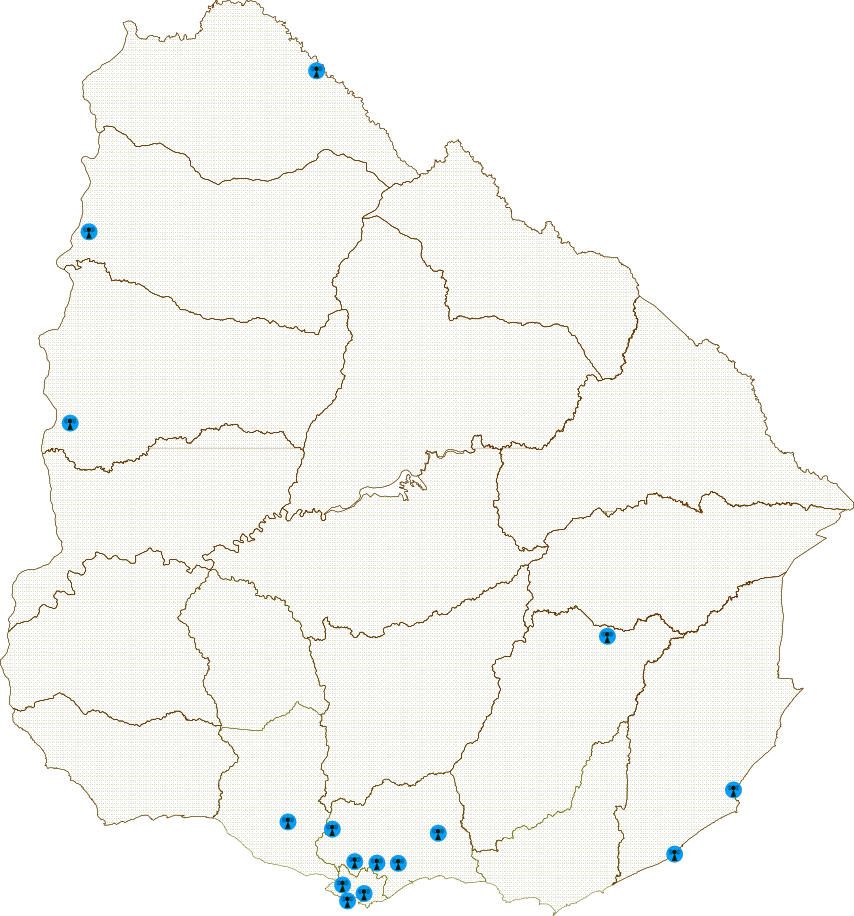
\includegraphics[scale=0.6]{./Cap/imestaud/MapaTotal.png}
 % MapaTotal.png: 854x916 pixel, 120dpi, 18.08x19.39 cm, bb=0 0 512 550
 \caption{Mapa de las radios comunitarias asociadas a AMARC que participaron en el proyecto de extensión universitaria Las Radios no son Ruido.}
 \label{MapaTotal}
\end{figure}

\subsection{Zona Norte}
\begin{figure}[htbp!]
 \centering
 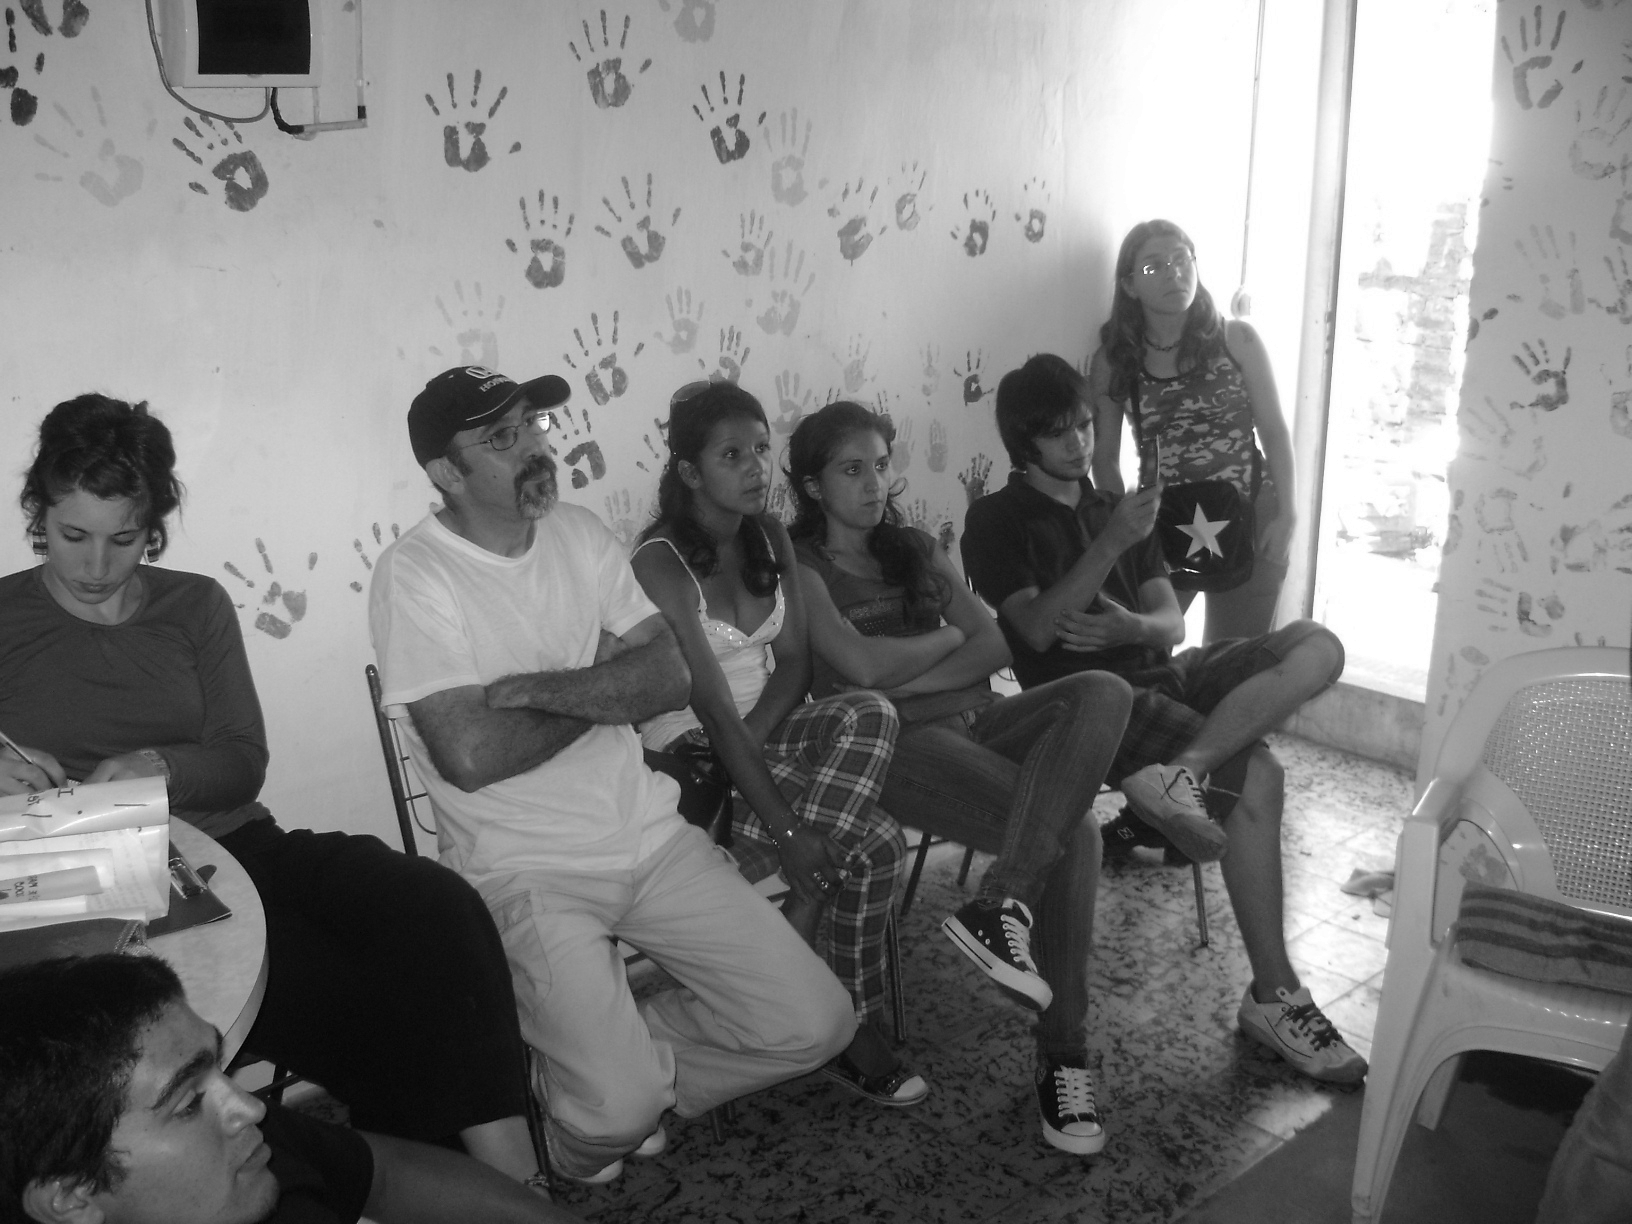
\includegraphics[scale=0.15,keepaspectratio=true]{./Cap/Fotos/HorizontePay.jpg}
 % HorizontePay.jpg: 1632x1224 pixel, 72dpi, 57.57x43.18 cm, bb=
 \caption{Taller en radio Horizonte, Paysandú.}
 \label{HorizontePay}
\end{figure}

\textbf{“Horizonte Max”. Artigas.} Se realizó el taller en un salón comunal, con gran parte del colectivo. En el mismo, los participantes hacen hincapié en la gran saturación de radios de tipo comunitario (aunque no comprendidas dentro del censo de URSEC), la problemática de relacionamiento con dichas radios, además de la recepción de radios brasileras, las cuales interfieren en la correcta recepción de señales propias del departamento.\\

\textbf{“Impactos”. Salto.} El lugar de trabajo fue el club social y deportivo La Paloma, donde se encuentran las instalaciones de la radio. El taller no se pudo instrumentar por la escasa asistencia del colectivo, realizando de modo parcial las tareas propuestas.\\

\textbf{“Horizonte”. Paysandú.} Se realizó el taller en la propia radio con gran participación de los miembros de la misma. Se trataba de un colectivo joven con gran receptividad a la propuesta.\\

\subsection{Zona Este}

\textbf{“Radio Parque”. La Paloma, Rocha.} El encuentro se realizó en las instalaciones de la vieja estación de AFE con dos integrantes de la radio, que actualmente sostienen el proyecto radial. Igualmente se pudo instrumentar el taller y posteriormente se realizaron las encuestas.\\

\textbf{“El Capiz”. Valizas, Rocha.} El taller se realizó en las instalaciones de la radio con la mayoría del colectivo, no así las encuestas, las cuales quedaron en manos de los integrantes de la radio para su posterior realización por iniciativa propia.\\

\textbf{“La Heladera”. José Pedro Varela, Lavalleja.} El taller se realizó en el local de la radio con gran participación del colectivo. En la realización de las encuestas colaboraron la mayoría de sus miembros.\\

\subsection{Montevideo, San José y Canelones}
\begin{figure}[htbp!]
 \centering
 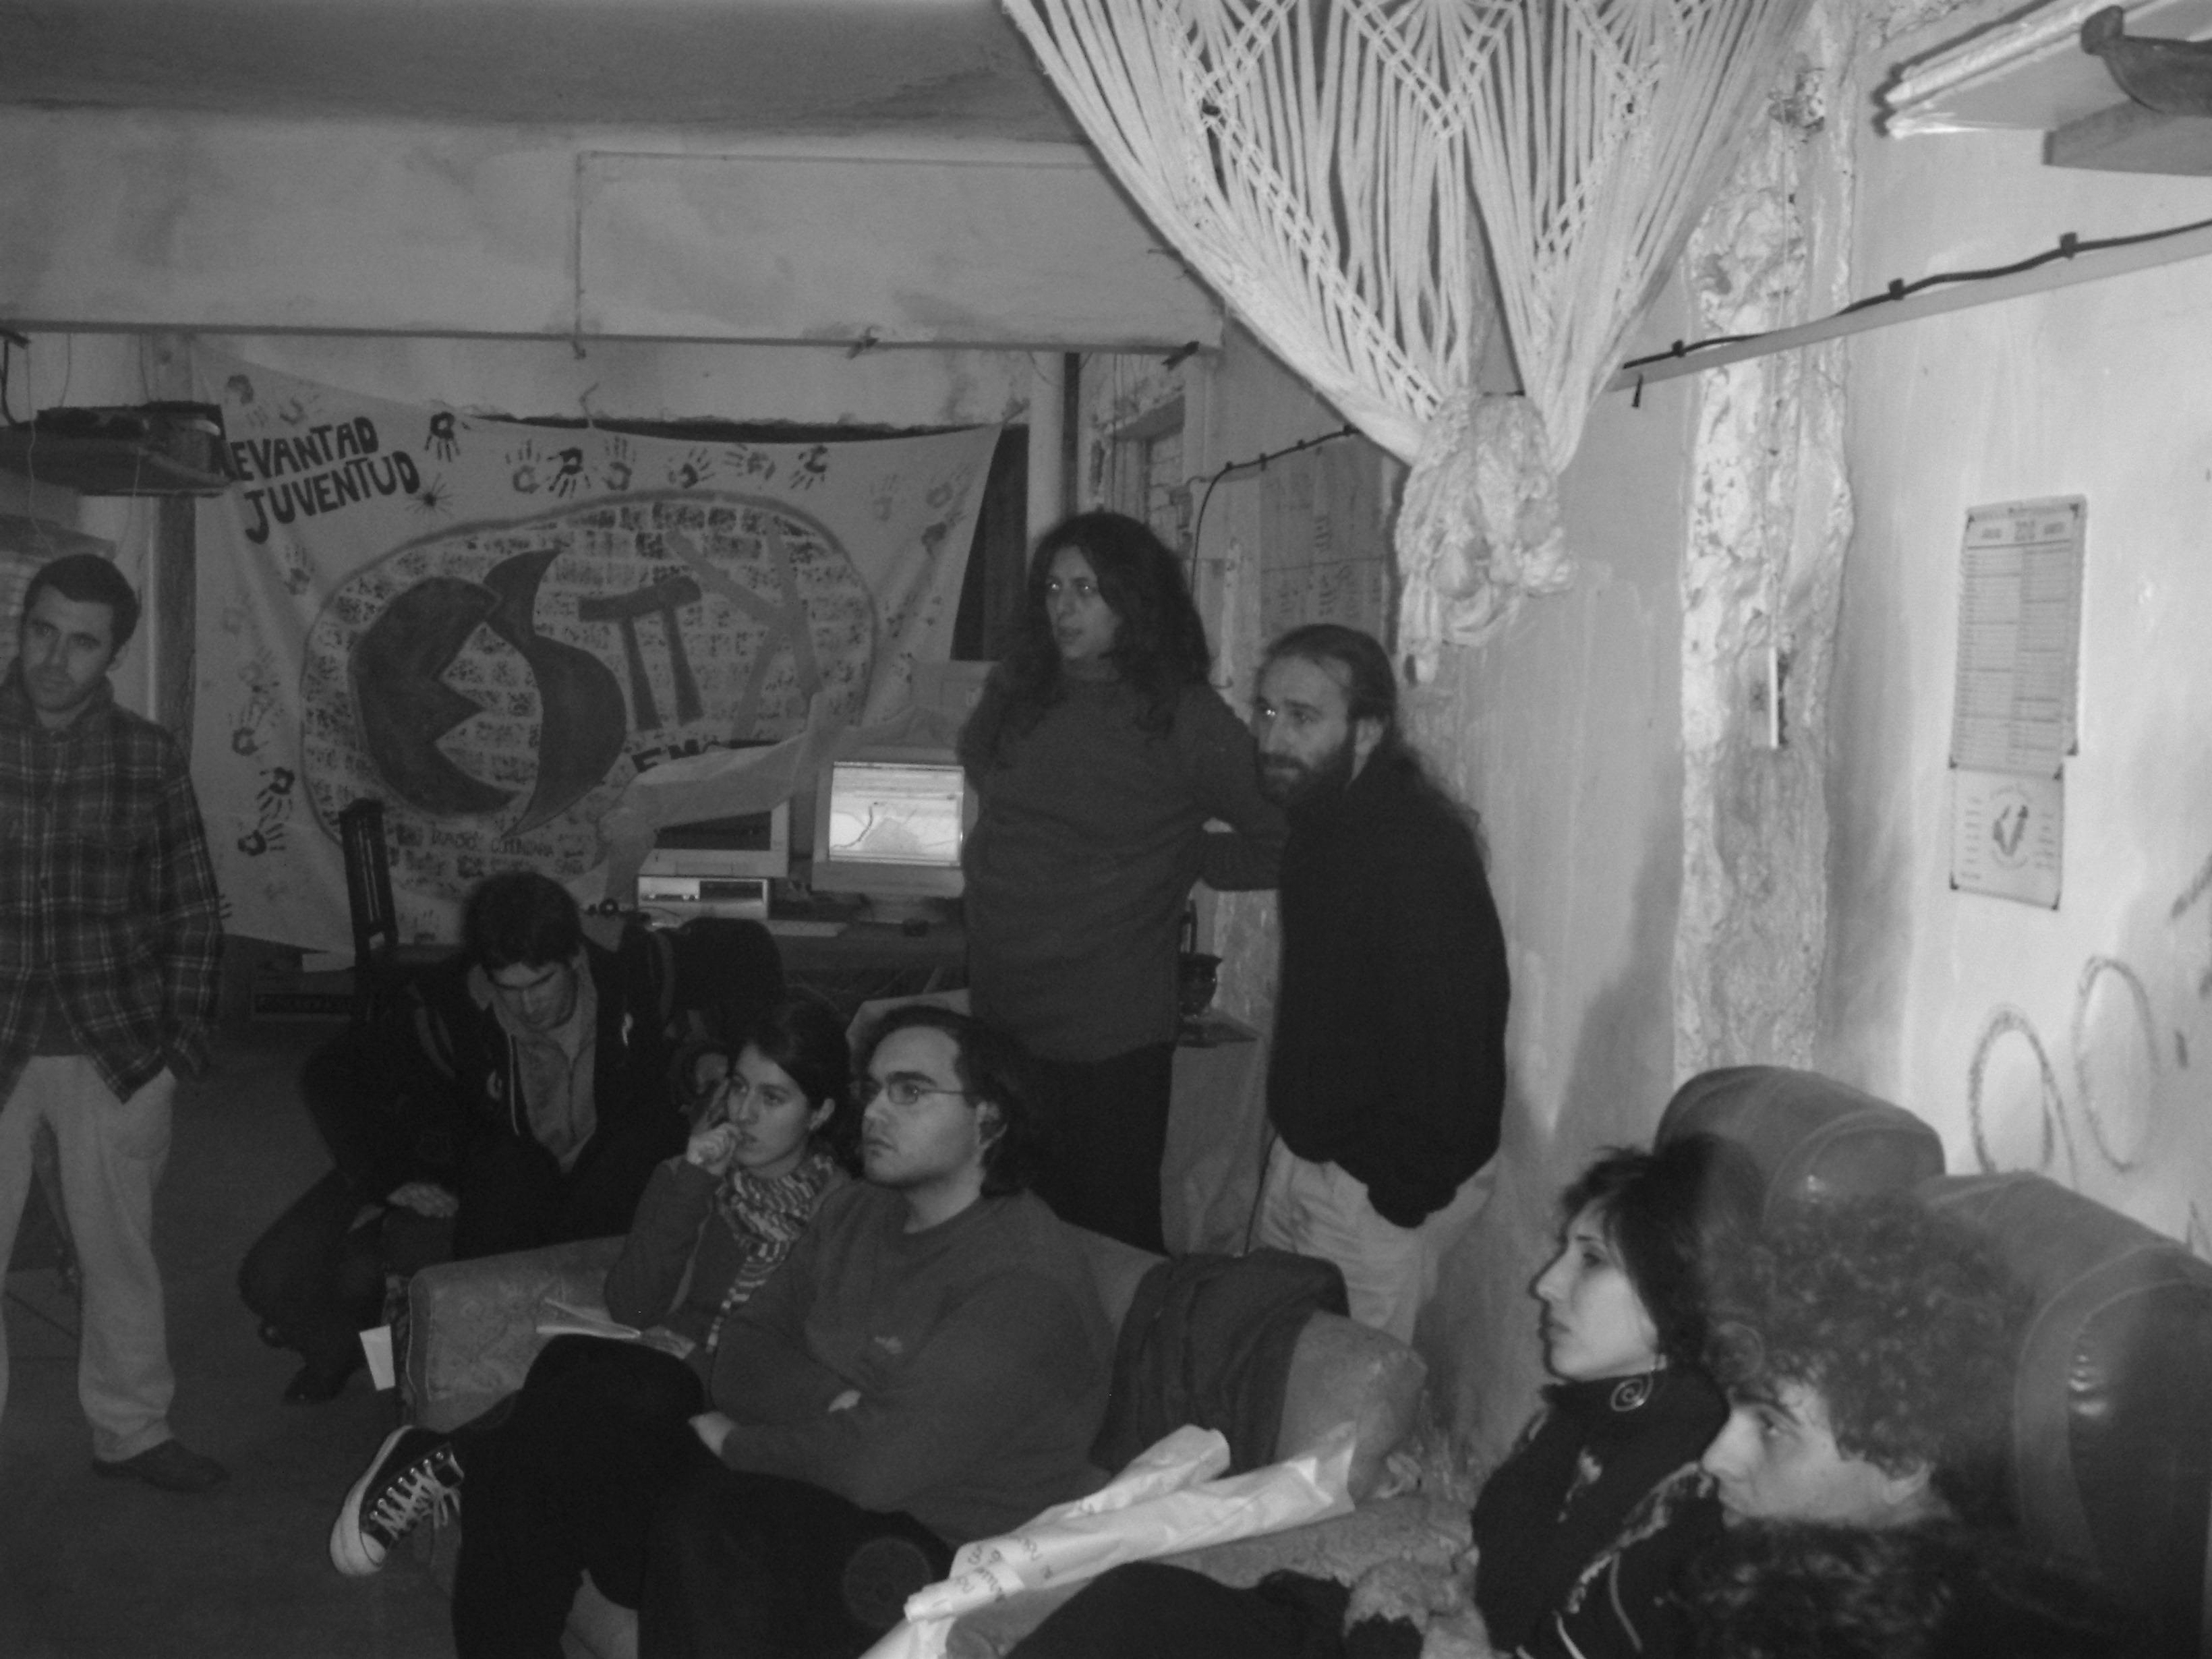
\includegraphics[scale=0.1,keepaspectratio=true]{./Cap/Fotos/Espikabyn.jpg}
 % Espikabyn.jpg: 3280x2460 pixel, 96dpi, 86.78x65.09 cm, bb=
 \caption{Taller en radio Espika, Santa Lucía, Canelones.}
 \label{Espika}
\end{figure}
\textbf{“Universo”. Montes, Canelones.} Se caracteriza por tener un colectivo numeroso y por ser la única señal de radio local. El taller se realizó con la mayoría de sus integrantes y las encuestas no tuvieron participación por parte de los miembros de la radio.\\

\textbf{“Radio Prado”. Paso de la Arena, Montevideo.} Se realizó una reunión previa al trabajo propuesto, dado que el colectivo había pasado por varios encuentros con otros proyectos universitarios con los cuales no habían tenido buenas experiencias. El encuentro se realizó en las instalaciones de la radio, ubicada en la casa de uno de los integrantes. Dicha reunión se caracterizó por una buena participación del colectivo de la radio, contando incluso con una integrante que se encontraba en Estados Unidos, que participó mediante teleconferencia.\\

\textbf{“Vilardevoz”. Reducto, Montevideo.} La primer actividad realizada fueron las encuestas con participación de integrantes de la radio. El taller se realizó dentro de las instalaciones de la radio las cuales se encuentran en el propio hospital. Colectivo numeroso compuesto por usuarios del hospital y el equipo técnico.\\

\textbf{“General Artigas”. Toledo, Canelones.} Se trabajó con un colectivo numeroso, el cual poseía una grilla muy variada en programación. La encuesta fue realizada por los integrantes de la radio en otra ocasión.\\

\textbf{“Espika”. Santa Lucía, Canelones.} El taller se realizó en las instalaciones de la radio, un local alquilado cerca del centro de la ciudad. El colectivo era pequeño, y participó en toda la actividad. La radio está inmersa en un proyecto multicultural el cual forma parte de distintas actividades artísticas y culturales. En la realización de las encuestas participaron integrantes de la radio.\\

\textbf{“Timbó”. San José.} El taller se realizó con la mayoría del colectivo y posteriormente se realizaron las encuestas en conjunto con integrantes de la radio. El grupo era pequeño y contaba con local propio, cedido por una cooperativa de vivienda.\\

\textbf{“Utopía”. Colonia Nicolich, Canelones.} La radio se ubicaba cerca del Aeropuerto Internacional de Carrasco. En una primera instancia se realizó la encuesta con participación de integrantes del colectivo. Posteriormente, se desarrolló el taller en el local de la radio el cual se ubicaba dentro del predio de la casa de uno de los miembros, con gran participación del colectivo.\\

\textbf{“La Cotorra”. Cerro, Montevideo.} El encuentro se realizó en el local alquilado de la radio con poca participación del colectivo. Se realizó en una primera instancia el taller y posteriormente con la colaboración de algunos de los integrantes se realizaron las encuestas.\\

\textbf{”Insomnio”. Las Piedras, Canelones.} En este caso no fue posible realizar el taller, por dificultades de coordinación, pero los integrantes del colectivo realizaron por su parte las dinámicas previstas y la totalidad de las encuestas, quedando incluidos en el relevamiento.\footnote{Al momento de la publicación de este material, Insomnio FM ya no es una radio asociada a AMARC.}\\
\begin{figure}[htbp!]
 \centering
 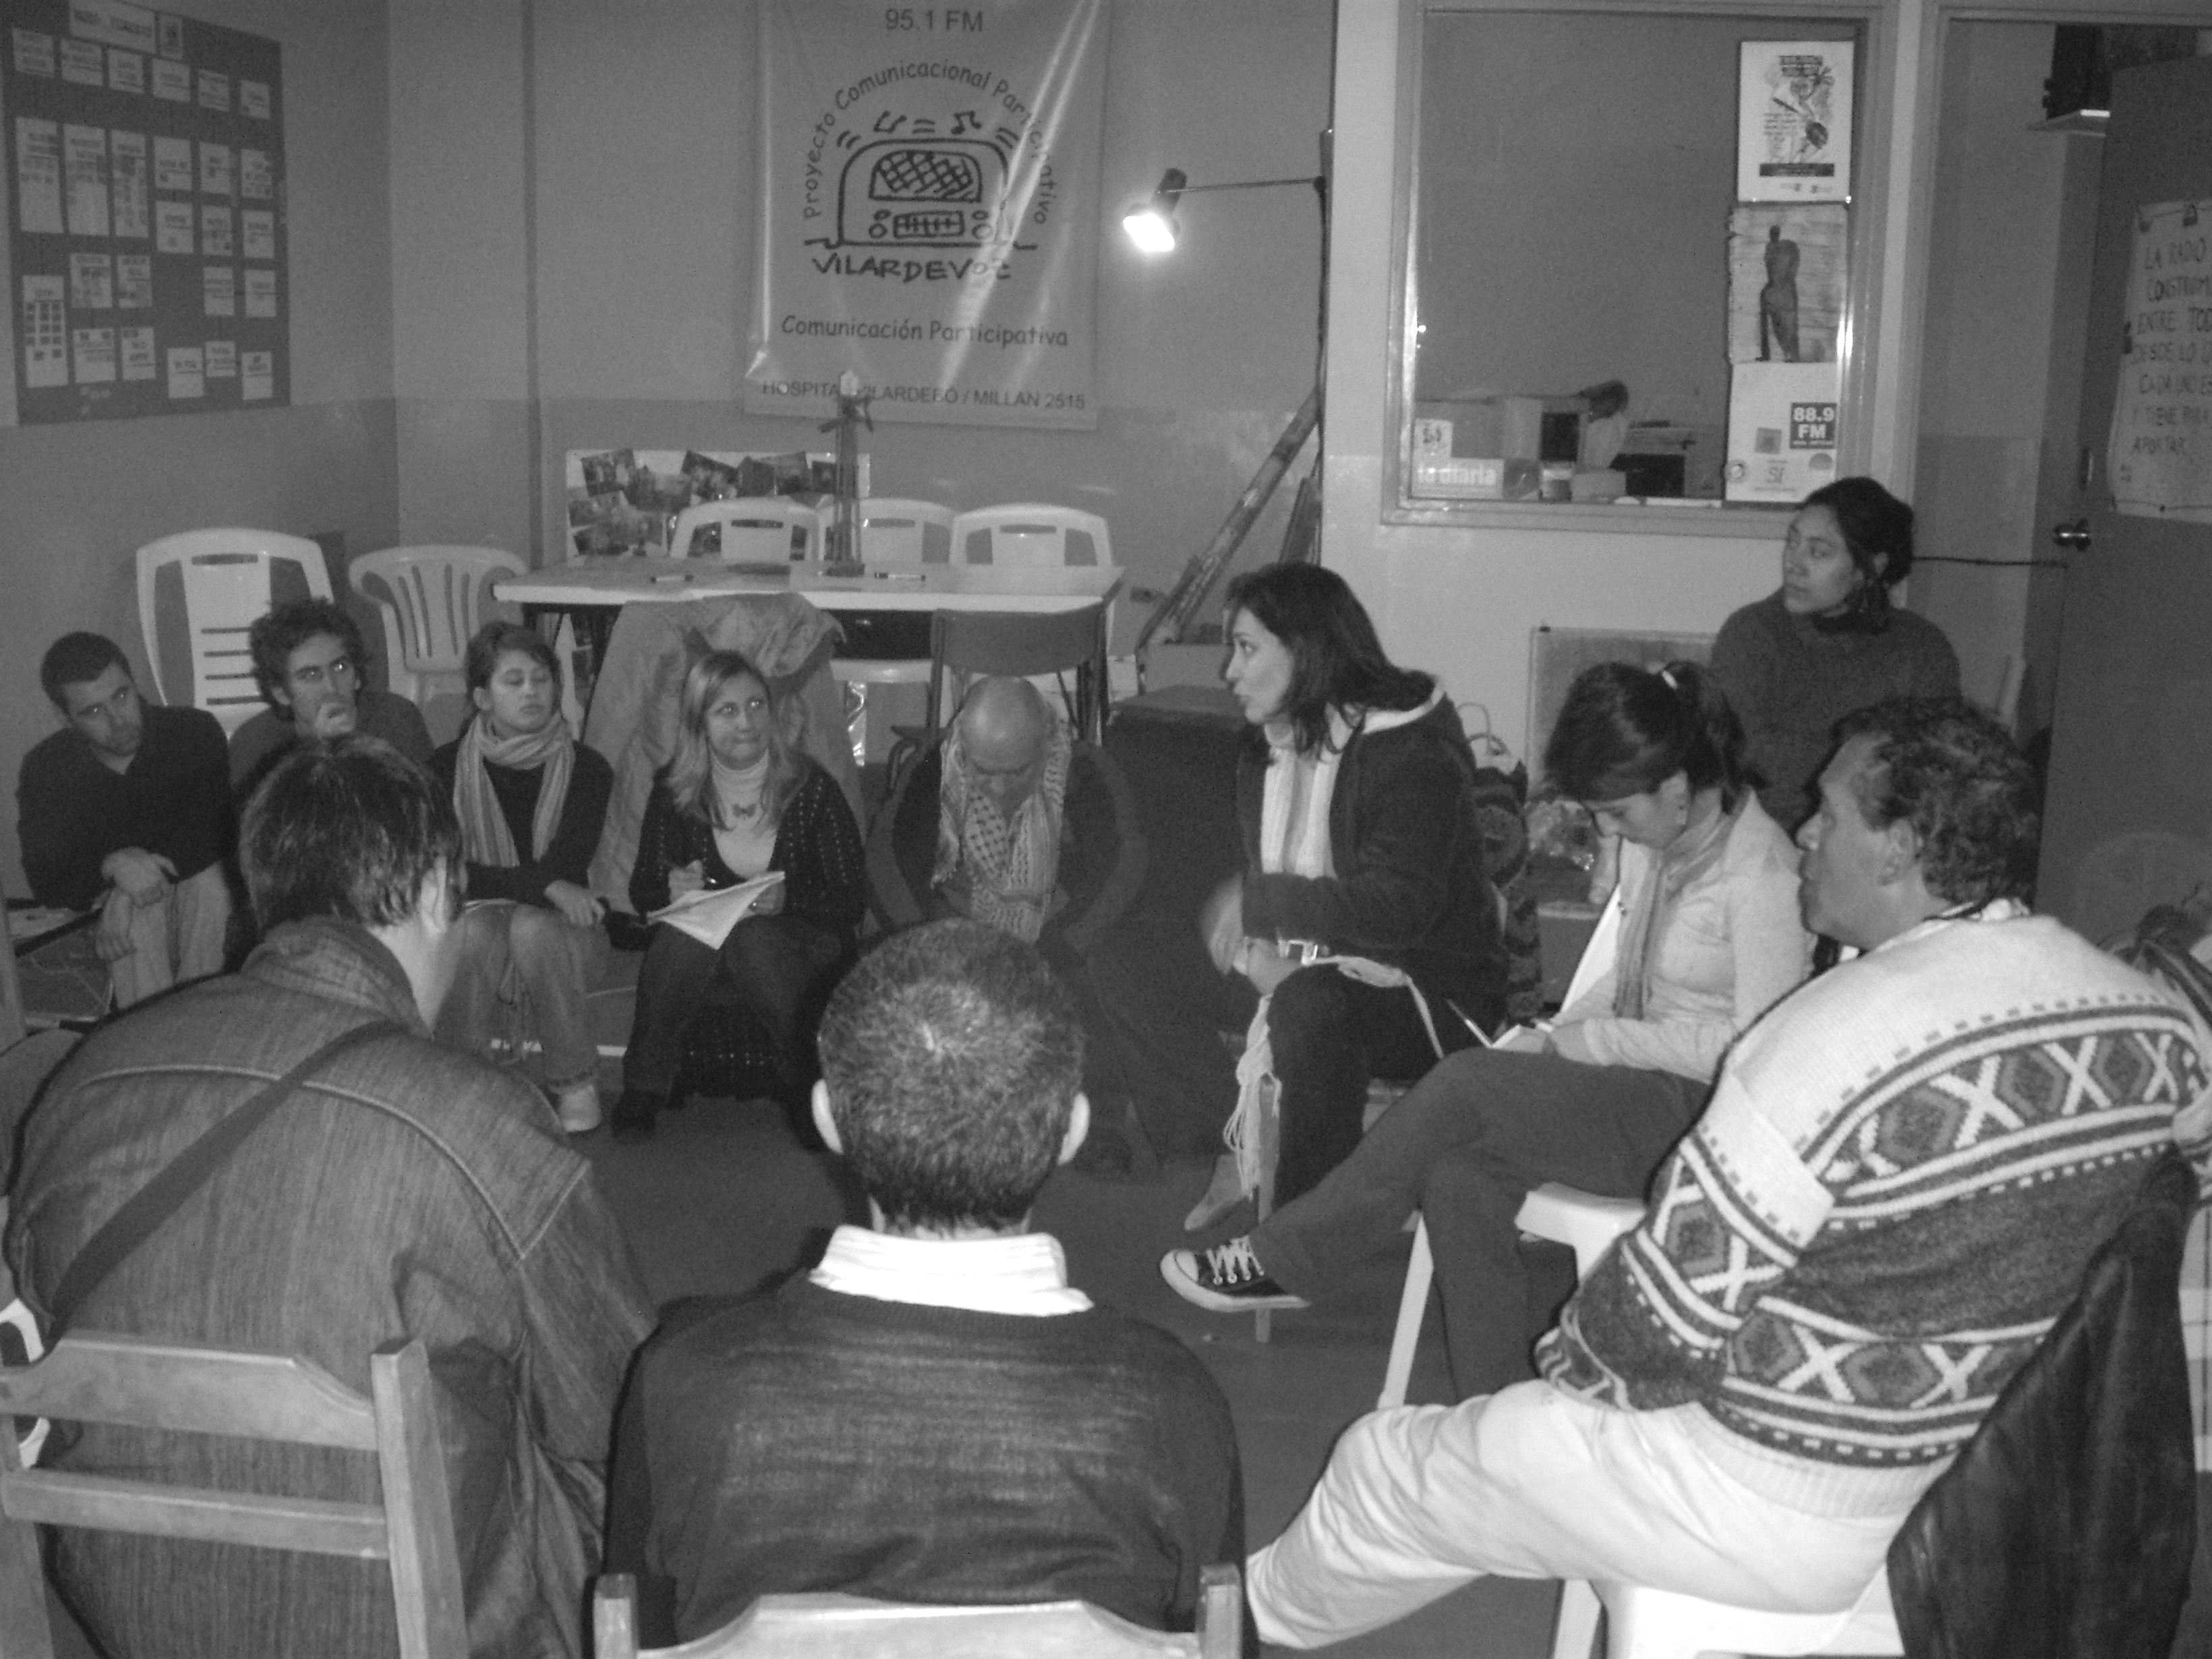
\includegraphics[scale=0.1,keepaspectratio=true]{./Cap/Fotos/Vilarbyn.jpg}
 % Vilarbyn.jpg: 3280x2460 pixel, 96dpi, 86.78x65.09 cm, bb=
 \caption{Taller en radio Vilardevoz, Hospital Vilardebó, Montevideo.}
 \label{Vilarbyn}
\end{figure}

Por otra parte, en el caso de la emisora “Ciudad” de Los Cerrillos (Canelones), se suspendieron los talleres acordados, puesto que la radio estaba en mudanza de local, no pudiéndose establecer nueva instancia de trabajo.\\

Es necesario destacar también que con la radio “El Puente”, La Teja (Montevideo), se realizaron diferentes contactos, pero no se logró realizar ni el taller ni las encuestas.\\

Asimismo, no fue posible relevar información de tres emisoras citadas en la membresía original brindada por AMARC, debido a que las mismas ya no se encontraban funcionando. Este es el caso de “La Gaviota” de Villa García (Montevideo), “Comunitaria” de Soca (Canelones) y “La Quimera” de Atlántida (Canelones).\\

\subsection{Taller nacional}

Se llevó a cabo en el local radial de “El Puente”. Al día siguiente del taller, AMARC tenía Asamblea General. La actividad tuvo alta participación, con al menos un integrante de la mayoría los colectivos. Se trabajó en pequeños grupos, donde cada equipo tenía un documento base, referido a la sistematización de lo relevado en esa área específica. Posteriormente, en plenario general, cada grupo discutió sobre su impresión del documento y relató los aportes que entendía oportunos. Este plenario hizo acuerdo con diversos aportes a ser incluidos en la publicación final. Luego, se realizó una presentación de los datos del Estudio de audiencia. Finalmente se realizó una evaluación del proceso y de los resultados, entregándose el material (papelógrafos y encuestas) a cada colectivo.
\part{Sistematización y colectivización de saberes}
\chapter{Introducción a la sistematización y colectivización de saberes}

Los siguientes documentos fueron realizados en base a los conocimientos que cada radio ha acumulado, a lo largo de su historia, en relación a su propia gestión. Incluye también parte de la historia de cada radio en sus aspectos fundacionales.\\

En la recolección de la información, así como en la discusión de los documentos, se trabajó en base a técnicas participativas, debido a que éstas permiten la discusión y reflexión colectiva. En base al conocimiento individual, los registros y memorias de cada integrante es que se constituye también la memoria colectiva, y en el trabajo en conjunto se potencia el conocimiento de todos.\\

El trabajo previsto en el encuentro con cada colectivo incluía la división de las tareas en equipos, cada uno con una temática diferente, y luego la realización de una instancia plenaria, donde cada grupo expone al resto de los participantes a efectos de complementar la información y realizar la síntesis colectiva de cada tema. En los casos donde los colectivos eran reducidos en número, no se realizó la división en equipos, trabajando en modalidad plenaria desde el principio.\\

Se utilizaron las mismas técnicas (una para cada área a relevar) en cada radio, para homogeneizar su sistematización. De esta forma fue posible una mejor organización de la información total relevada a nivel de toda la red.\\

Como referencia se tomó también el cuaderno bitácora (del equipo universitario) donde se registraba cada encuentro, para aclarar o complementar información.\\

Los documentos que siguen a continuación son una sistematización posible del vasto material recogido. Es la organización más adecuada, respetuosa y clara que el equipo universitario encontró para la presentación del material.\\

Todos los documentos fueron presentados a la red, trabajados en el taller nacional, discutidos y aprobados en la instancia plenaria. Posteriormente se recogieron los aportes y modificaciones sugeridas por los colectivos en dicha instancia.
\chapter{Recursos financieros\label{financieros}}

\section{Socios}

Se considera socio colaborador aquella persona que contribuye al sustento del colectivo mediante una aportación monetaria mensual. Es la fuente de financiamiento más genuina, por hacer parte a la comunidad en el sustento económico del proyecto radial. Resulta oportuno destacar que ser colaborador no implica ser miembro activo, aunque si puede ejercer el derecho por la propia definición de comunitaria de las radios.\\

Menos de la mitad de las radios visitadas instrumenta este sistema. Lo hacen mediante el cobro de una cuota que oscila entre los $\$$10 y $\$$50 de forma mensual o bimensual. Quien se encarga de la cobranza por lo general es un compañero del colectivo y retira para sí un porcentaje del dinero cobrado a modo de comisión.\\

En el caso de Radio Horizonte Max de Artigas cada comunicador es socio colaborador. En Radio Timbó sus integrantes colaboran también con aportes mensuales.\\

En La Cotorra se llegó a un acuerdo con una compañera del colectivo con experiencia en ventas y marketing para que se encargara de la captación y fidelización de socios.\\

\section{Publicidad}

La publicidad es una forma destinada a difundir o informar al público sobre un bien o servicio a través de los medios de comunicación con el objetivo de motivarlos hacia una acción de consumo.\\

De las radios relevadas, casi la totalidad ofrece publicidad. De lo recaudado, el principal destino es el sustento económico del colectivo, básicamente para el pago de gastos generales.\\

Por lo general, se cobran cuotas de bajo monto y son a comercios locales o “comercios amigos” a los cuales se le efectúan canjes (tanto en bienes como en servicios) o el propio cobro contado.\\

Los avisos publicitarios salen distintamente al aire dependiendo del importe que abona y de las pautas que se establecieron en cada colectivo. La modalidad instrumentada varía en cada uno de ellos, va desde quienes mencionan 6 avisos por programa hasta quienes sólo sacan 4 en el correr del día.\\

En el caso de Radio Espika, sólo se ofrece publicidad cuando se realizan eventos. Lo recaudado se destina para financiar los posibles costos de cada evento, como por ejemplo el sonido. Actualmente es una de las radios que se encuentra sin vender publicidad y viene atravesando un largo proceso de discusión al respecto. Se viene evaluando los contenidos de las publicidades y las características de cada auspiciante, ya que entienden que la publicidad que se transmite es parte del contenido de la radio.\\

La venta de publicidad es el recurso financiero que mayor discusión genera dentro del colectivo. Los proyectos de las radios comunitarias no tienen fines de lucro, lo cual no significa ir a pérdidas. Les resulta necesario lograr la sustentabilidad económica en el tiempo. Es así que surge la discusión sobre cómo debería instrumentarse este recurso financiero. Cómo vender publicidad, con qué contenido, bajo qué condiciones y quiénes serían los auspiciantes.\\

Los colectivos que hoy no venden publicidad están trabajando en ello. Unos estudiando la zona y los posibles comercios a los que se les podría vender y si bien otros ya tienen previsto el procedimiento de venta, están esperando a mejorar su programación.\\

\section{Recursos estatales}

Aunque en general se trata de proyectos financiados por entidades estatales, también existen algunos casos de trabajo con recursos de otros tipos de organismos, como el Programa Naciones Unidas para el Desarrollo (PNUD). Menos de la mitad de los colectivos han acudido a financiar algún proyecto con fondos del Estado. Es el caso de El Capiz de Valizas, Espika FM de Santa Lucía, Insomnio de Las Piedras, La Cotorra y Vilardevoz de Montevideo y Radio Horizonte de Paysandú.\\

El Capiz postuló un proyecto a los fondos vecinales de la Intendencia Municipal de Rocha. Son recursos destinados a promover el desarrollo de la región. El proyecto presentado por la radio no resultó aprobado.\\Link: \href{http://www.rocha.gub.uy}{www.rocha.gub.uy}.\\

Los compañeros de Espika presentaron en el año 2009 un proyecto a los Fondos Concursables del MEC. El mismo consistía en el trabajo conjunto de estudiantes de tercer año de liceo de las localidades de Santa Lucía, Los Cerrillos y 25 de Agosto. Los docentes participantes del proyecto donaron parte de sus honorarios a efectos de continuar con la construcción de un espacio socio-cultural.\\Link: \href{http://www.fondoconcursable.mec.gub.uy}{www.fondoconcursable.mec.gub.uy}.\\

Radio Vilardevoz trabaja actualmente con estudiantes de Facultad de Psicología, quienes realizan sus pasantías curriculares de cuarto y quinto ciclo participando en los diferentes espacios de trabajo del colectivo. En el mismo se cuenta con el apoyo de una docente de la facultad mencionada con la función de enseñanza. Asimismo, se vienen realizando algunas actividades específicas financiadas por CSEAM (Comisión Sectorial de Extensión y Actividades en el Medio), como por ejemplo el financiamiento de un desembarco en Psicología en noviembre de 2010.\\Link: \href{http://www.extension.edu.uy}{www.extension.edu.uy}.\\

La Cotorra tuvo una experiencia con el PNUD. La misma propuso como objetivo general aportar a la recuperación de la memoria reciente tomando como referente a los protagonistas del barrio (Cerro de Montevideo) intentando reflejar en ellos a la comunidad toda. Se desarrolló desde marzo a octubre 2009.\\Link: \href{http://www.undp.org.uy/pnuduruguay}{www.undp.org.uy/pnuduruguay}.\\

Insomnio postuló un proyecto al INJU (“Entre Jóvenes”) en el programa Amplifica tu Voz, el cual fue aprobado en el año 2010. El mismo tiene como objetivo general financiar el arreglo de la sede social (pintar y colocar un cartel en el frente) y conseguir una consola para la radio. \\Link: \href{http://www.inju.gub.uy}{www.inju.gub.uy}.\\

En el caso de Radio Horizonte de Paysandú, se postuló un proyecto al Presupuesto Participativo de esa localidad, el cual solicitaba híbridos, computadoras y consola. No se contó con los votos suficientes para que fuera aprobado. Entre otras estrategias, realizó una campaña vía mensajes de texto.\\Link: \href{http://www.paysandu.gub.uy}{www.paysandu.gub.uy}.\\

Existe el caso de un colectivo que no está de acuerdo con el apoyo estatal a las radios comunitarias.\\

\section{Otros}
El colectivo Espika de Santa Lucía es uno de los que más ha desarrollado la búsqueda de fondos alternativos para financiamiento.
Actualmente, cuentan con cuatro fuentes de ingresos provenientes de:
\begin{itemize}
 \item Cantina y entradas a eventos culturales
 \item Coproducciones como presentación de libros, discos y obras de teatro
 \item Distribución de La Diaria
 \item Distribución de música independiente (discografía)
\end{itemize}

\indent Casi la totalidad de los colectivos recibe una colaboración proveniente del bolsillo de cada miembro. Varias se financian también con rifas, bailes, eventos artísticos, varietés, venta de comida, canjes y bonos colaboración. Reciben asimismo donaciones puntuales (sillas, estufas o dinero para acondicionamiento del local). Hay un colectivo que se encarga de reciclar material de los lugares de trabajo de algunos de los miembros, como ser computadoras, impresoras y muebles.
\chapter{Aspecto técnico\label{tecnico}}

\indent En cada una de las radios visitadas, se trabajó el aspecto técnico utilizando un papelógrafo, donde se relevaban problemas frecuentes y sus soluciones, el paso a paso de la solución de un problema específico, los materiales utilizados y los referentes técnicos. La intención era generar una especie de “manual técnico” de radios, escrito por radialistas para radialistas, tomando como base la experiencia de años de trabajo. Durante la redacción de este proyecto (mayo-junio de 2009), se había visto que el tema técnico era de suma importancia para los colectivos, y por eso se lo tomó como un aspecto a trabajar.\\

En las visitas a las radios, se encontró que, en general, no existían grandes problemas técnicos, o problemas con una solución muy compleja. Incluso, en muchas radios no pudo elaborarse el paso a paso de la solución a un problema técnico específico, dado que los problemas presentados parecían de solución simple para los participantes. En algunos casos particulares, existían varios integrantes del colectivo con mucha preparación y experiencia en lo técnico, pero no es la generalidad. Por otra parte, uno de los grandes temas en lo técnico refiere al uso de software libre. Aunque AMARC Uruguay tomó en asamblea la decisión política de usar software libre en las radios, la instrumentación en la red no se ha completado aún.\\

De todos modos, resultaría aventurado concluir que no existen problemas técnicos en las radios. Quizá la metodología usada en los talleres no sirvió para poder relevarlos de manera adecuada. También hay que resaltar que la implementación del proyecto Laboratorio TICs cambió sustancialmente la realidad de muchas radios, dotándolas a todas de un equipamiento mínimo (consola, computadora, micrófono) de buena calidad. Existe una valoración muy positiva del Laboratorio TICs, en relación al aporte de infraestructura; mas, en lo relativo al aprovechamiento de la misma, se señala un gran debe (desconocimiento de Ubuntu, uso no eficiente de consolas).\\

Se realizó una clasificación del conjunto de problemas técnicos relevados en los talleres. Los grandes bloques de problemas técnicos refieren a:

\begin{enumerate}
  \item Problemas eléctricos (instalación, descargas, cortes de energía)
  \item Relacionados con la informática (linux, desprogramación de tandas, salida por internet, cuelgues de computadoras)
  \item Comunicación con el exterior (audiencia, cobertura de eventos)
  \item Salida al aire (micrófonos, saturación, salida en estéreo, calidad de sonido, amplificación)
  \item Transmisión (poca potencia, antena, interferencias con radios y TV, alcance)
  \item Capacitación (software libre, técnica en general, manuales engorrosos)
\end{enumerate}


Dentro de cada uno de los temas, existen problemas que se reiteran, por constituir parte del día a día de las radios, y otros que son únicos y circunstanciales. Algunos no son solucionables en la interna, sino que se solucionan mediante la adquisición de equipos nuevos, por lo cual se omiten en este resumen.\\

Analizaremos cada bloque de problemas por separado.

\section{Problemas eléctricos}

\indent Uno de los problemas presentados fue el estado precario de las instalaciones eléctricas de algunas radios. Debido a las exigencias asociadas a la legalización de las radios comunitarias, este problema ha sido solucionado (o está en vías de solución), para la mayor parte de los colectivos, puesto que es uno de los puntos estudiados por la inspección de la URSEC\footnote{Unidad Reguladora de los Servicios en Comunicaciones: \href{http://www.ursec.gub.uy}{www.ursec.gub.uy}}. Dado que el aterramiento es parte de lo requerido en la instalación, el problema de las descargas se encontraría mitigado.\\

Los cortes frecuentes de energía fueron comentados por dos radios de Canelones (General Artigas y Universo). La solución pasa por instalar una UPS\footnote{Uninterruptible Power Supply: Suministro ininterrumpible de energía} y un equipo generador, que supla de energía a la radio hasta el restablecimiento de la de UTE.\\

\section{Informática}

\indent Un problema frecuente era el cuelgue de la computadora usada para salir al aire. Como solución transitoria, algunos compañeros usan un reproductor de música (antiguamente un discman, ahora reproductores de mp3) para salir al aire mientras reiniciaban el equipo.\\

\indent Los virus en las computadoras constituyen otro problema usual. Estos son llevados por los pendrives o reproductores de mp3 y mp4, que a su vez son infectados en computadoras de acceso colectivo (familiares, cybercafés, etc). Un virus es básicamente un programa que se ejecuta sin el control del usuario, para realizar tareas variadas: desde borrar información hasta extraer información confidencial de los usuarios (números de tarjetas de crédito, contraseñas, etc) y enviarlas por internet. Se instala en la computadora porque es ejecutado por el programa de reproducción automática de Windows (cuando se conecta un pendrive, aparece una ventana preguntando qué se quiere hacer con el mismo).\\

Existen varias formas de evitar este problema:

\begin{enumerate}
  \item Usar Linux (Ubuntu, por ejemplo) como sistema operativo, en lugar de Windows, donde no se registran problemas con virus.	
  \item Desactivar la reproducción automática de dispositivos USB. Dependiendo de la versión de Windows, existe una opción de deshabilitar que se autoejecute el contenido del pendrive (que puede ser un virus).
\end{enumerate}


\indent Como se mencionó anteriormente, existen algunos problemas con el manejo de Linux en las radios. El principal refiere a la falta de conocimiento de programas para radio en Linux, es decir, una aplicación que permita crear una lista de archivos de sonido de duración total conocida, de modo de saber entre qué horas va a ser emitida. El programa comúnmente usado para salir al aire es el ZaraRadio, que es software libre (código abierto para poder ser modificado libremente), pero sólo funciona en Windows. Una solución comúnmente encontrada para usarlo en Linux es a través de la aplicación Wine, que permite correr programas para Windows bajo Linux. Otra alternativa es directamente utilizar otra aplicación, del género de reproducción de archivos de sonido, como el Audacity\footnote{\href{http://audacity.sourceforge.net/?lang=es}{audacity.sourceforge.net/?lang=es}}. Existen también proyectos de programas de código abierto para radios, como el Rivendell\footnote{\href{http://www.rivendellaudio.org}{www.rivendellaudio.org}} o el Internet DJ Console \footnote{\href{http://sourceforge.net/projects/idjc/files}{sourceforge.net/projects/idjc/files}}.\\

En una radio (La Heladera) no podían entrar a internet directamente desde la computadora con Linux, lo cual se solucionaría instalando un router (que además, por ser inalámbrico, proporcionaría acceso a la red desde el exterior, como sucede en radio Prado para los niños que tienen XO).\\

En relación a la informática, otro tema es la salida a través de internet. Como muestra el estudio de audiencia, existe un alto porcentaje de la población que tiene acceso a la red. Además, cada vez es más común escuchar radio por internet. Incluso las computadoras del Plan Ceibal vienen con un programa para escuchar radio: Ceibal Radio, desarrollado por la asociación civil uruguaya CeibalJAM!\footnote{\href{http://ceibaljam.org}{ceibaljam.org}}, donde ya aparece una de las radios comunitarias asociadas a AMARC: Radio Prado.\\

Todas las radios visitadas participan del podcast de AMARC\footnote{\href{http://podcast.amarcuruguay.org}{podcast.amarcuruguay.org}}, subiendo archivos de audio con emisiones. Pero muchas no emiten por internet en tiempo real todavía, por falta de recursos financieros o de conocimento de formas gratuitas de transmisión. En el capítulo \ref{Comunica} se puede ver la lista de radios que emiten en internet en tiempo real (a diciembre de 2010).\\
% 
% Las radios que transmiten en tiempo real por internet son:
% 
% \begin{itemize}
%   \item Radio Gral Artigas: \url{http://radioartigas.listen2myradio.com}
%   \item Radio Vilardevoz: \url{http://www.ustream.tv/channel/transmisiones-vilardevoz}
%   \item Radio Horizonte Max: \url{http://horizontemax913.blogspot.com}
%   \item Radio Prado: \url{http://www.elpradofm.net/transmitiendo.html}
%   \item Radio Horizonte: \url{http://www.horizonte989.org/radio}
%   \item Radio Universo: \url{http://www.ustream.tv/channel/radiouniversofm}
% \end{itemize}

\section{Comunicación con el exterior}

Como se detalla en el punto de Comunicación con la Comunidad, existen varios medios de comunicación con la audiencia al aire, como las llamadas telefónicas, sms, correo electrónico, chat, etc. El más complejo es el pasar llamadas telefónicas al aire, para lo cual existen, al menos, dos alternativas de uso común:

\begin{enumerate}
  \item Usar manos libres de un celular
  \item Usar un teléfono híbrido
\end{enumerate}

El primer caso requiere un celular con línea, dedicado específicamente a la tarea de salir al aire. En el segundo, se puede realizar de manera artesanal el circuito, con muy bajo costo. Existen muchas versiones de circuitos para recepción y emisión de llamadas telefónicas\footnote{\href{http://www.proyectoelectronico.com/varios/hibrido-telefonico-phone-patch.html}{www.proyectoelectronico.com/varios/hibrido-telefonico-phone-patch.html}}.\\

Además de comunicación en vivo con la audiencia, otro problema es la transmisión de eventos públicos, como partidos de fútbol, festivales, tablados, etc. La solución más usual encontrada es usar un celular tarjetero, con llamadas gratuitas al teléfono de la radio. Otra es directamente usar una consola portáti.\\

\section{Salida al aire}

En este tema, se señalaron desde problemas circunstanciales (cables de micrófonos averiados, no salida en estéreo, etc; detectables con un tester y solucionables con un soldador) hasta otros más generales, relativos a mejorar la calidad del sonido (procesador de audio y codificador estéreo).\\

El problema de la saturación a la salida se soluciona con un correcto manejo de la consola (Espika: chequear que todos los vúmetros no estén saturando ni bajos al final de cada transmisión), al igual que la amplificación. Varias radios hablaron de tener un sonido que las \textit{distinguiera}, un sonido característico de cada radio, lo cual descansa en la tarea de los operadores.\\

Los problemas de ruido (``estática''), se deben a que el circuito del audio no está bien aislado. Por ejemplo, si los cables no están blindados (no tienen una malla protectora a tierra), pueden hacer de ``antena''. La calidad de las tierras es muy importante también (instalación de jabalinas).\\

El subaprovechamiento de la consola fue señalado en varias ocasiones. Existen compañeros que, por otro lado, explicitan que la aprovechan al máximo, como sucede en La Heladera.\\

Un dato no relevado fue si todas las radios salen en estéreo o no.\\

Varios colectivos señalan problemas con la aislación acústica, que generalmente es de fabricación casera (cajas de huevos). Muchas radios tienen la cabina cerca de la calle, lo que genera distorsiones por el ruido externo, mientras que otras ni siquiera tienen cabina. En el caso particular de Utopía, en Colonia Nicolich, la cercanía con el aeropuerto ocasiona grandes problemas acústicos.\\

\section{Transmisión}

Se mencionaron problemas con la antena. Algunas radios (Horizonte Max, Impactos) comentaron que tienen poco alcance, lo que sería solucionable si se aumentara la potencia permitida por parte de la URSEC (aunque eso podría generar interferencias con otras emisoras). Además sufren interferencia de otras emisoras, no siempre legales. En el interior, aparecieron varios casos de interferencias (con otras radios, TV), ruido en el transmisor.\\

\section{Capacitación}

\indent Un tema colateral que fue señalado en repetidas ocasiones, fue la formación técnica. En algunos colectivos (La Cotorra, Utopía, Horizonte, Espika) es habitual realizar instancias de formación, por medio de un compañero que ha aprendido sobre un tema específico (por ejemplo, uso de una nueva consola). También se realizan procesos de aprendizaje progresivo, donde un integrante del colectivo comienza colaborando en tareas técnicas sencillas, aumentando la complejidad con la experiencia adquirida. En otros (Horizonte Max), existen compañeros que no tocan la computadora ni la consola por ``miedo''.\\

\indent Otros colectivos (Parque, El Capiz, por ejemplo), hablaron de la falta de formación técnica. En ocasiones, se adquiere nuevo equipamiento, pero sin los respectivos manuales. Lo más habitual es que, cuando hay manuales, no sean leídos o no se entiendan (``precisamos manuales más sencillos'', La Cotorra).\\

\indent Con respecto al software libre, también se aprecia una falta de formación para utilizarlo. En primera instancia se debería pensar en el aprendizaje de un sistema operativo libre sencillo (como por ejemplo, Ubuntu, instalado en las computadoras del proyecto Laboratorio TICs), para luego pasar a programas más específicos para realizar edición y salir al aire.\\

\newpage
\section{Referentes técnicos}

\subsection{Generales}

\begin{itemize}
 \item José Imaz (La Cotorra)
 \item Daniel López (Capiz)
 \item Sebastián (Horizonte)
 \item Orlando (Horizonte)
 \item Carlos (Prado)
 \item Bruno Brian (Espika)
 \item Carlos Dárdano (Espika)
 \item Mauricio Torino (Espika)
 \item Nicolás Verdier (Espika)
 \item Víctor (Vilardevoz)
 \item Heber (Vilardevoz)
\end{itemize}


\subsection{Antena y equipos}
\begin{itemize}
 \item Daniel (Horizonte Max)
 \item Luis Malletti (La Heladera)
 \item Alfredo (Prado)
 \item Joan (Prado)
 \item Emir (Prado)
 \item Martín Acosta (Gral Artigas)
 \item Manuel Castelo (Gral Artigas)
 \item Hebert Madera (Utopía)
 \item Manuel (Utopía)
 \item Alejandro (Insomnio)
\end{itemize}

\subsection{Informática}
\begin{itemize}
 \item Rodrigo (Horizonte Max)
 \item Daniel Dutra (La Cotorra)
 \item Federico (Horizonte)
 \item Alejandro (Impactos)
 \item Esteban Yepor (La Heladera)
 \item Rodolfo Salvarey (Universo)
 \item Marcelo (Universo)
 \item Eduardo (Universo)
 \item Pablo Maulilla (Gral Artigas)
 \item Pablo Mass (Utopía)
\end{itemize}

\subsection{Edición, audio, salida al aire}
\begin{itemize}
 \item Diego Gómez (La Cotorra)
 \item Esteban Yepor (La Heladera)
 \item Javier Apolinario (La Heladera)
 \item Jorge Daniel Garro (Universo)
 \item Ariel Camacho (Utopía)
\end{itemize}
\chapter{Aspecto organizacional}

\section{Introducci\'on}

Del relevamiento realizado en los talleres, se desprenden determinadas formas de organización interna, enmarcadas en las distintas realidades de los colectivos que las conforman, pero que comparten la gestion colectiva y la búsqueda de la horizontalidad en la toma de decisiones. Asimismo, la creación de la ley Nº 18.232 (Servicio Radiodifusión Comunitaria) provee el marco legal correspondiente, el cual genera una serie de derechos y obligaciones, que necesariamente condicionan de una forma u otra a la organización en sí misma.\\

Dentro de este marco legal, la ley considera a las Asociaciones Civiles sin fines de lucro con personería jurídica reconocidas por el Ministerio de Educación y Cultura o en trámite de constitución, también aquellos grupos de personas organizadas sin fines de lucro con iniciativas de carácter comunitario.\\

\section{Estructura (figura interna)}

\indent El estudio realizado permite dar cuenta de un universo diversificado en el cual conviven tanto sistemas organizacionales con estructuras claramente jerarquizadas (Asociación Civil) compuestas por directores, secretarios, coordinadores, tesoreros, etc; y otros con estructuras no tan elaboradas como las comisiones de vecinos. Si bien en una primera instancia se puede interpretar en el caso de las estructuras más complejas cierta rigidez, la información recabada también ha permitido entender que todas estas figuras que componen los diferentes organigramas organizacionales pretenden funcionar basados en la horizontalidad para la toma de decisiones. Cabe destacar que la capacidad referencial de ciertos integrantes de los colectivos ya sea por antigüedad, por saberes específicos, o por su capacidad de liderazgo funciona muchas veces como guía en la toma de decisiones del resto de los integrantes, lo que no significa que dichas decisiones no se pongan a consideración de la totalidad de colectivo.\\

En la mayoria de las radios comunitarias la organización interna dista de la figura legal, siendo más horizontales y flexibles que la forma jurídica que tienen que adoptar para existir legalmente. 
% Tanto las Asociaciones Civiles como las comisiones de vecinos son instrumentos de participación funcional, esta salvedad no es menor ya que justamente lo que muestra es el carácter de fluidez dentro de la organización, a saber, dichas estructuras no son respetadas a rajatabla en el funcionamiento sino más bien como una herramienta.

\section{Funcionamiento}

Se trabaja a través de asambleas ordinarias o extraordinarias en las cuales participa la totalidad del colectivo o en algunos casos los integrantes de la comisión directiva; donde se ponen en consideración los diferentes puntos a tratar. La periodicidad de dichas asambleas varía. Algunos colectivos realizan asambleas ordinarias de forma semanal, quincenal, mensual, otros una o dos veces al año. Lo mismo sucede con la elección de las distintas autoridades que componen tanto a las asociaciones como a las comisiones los tiempos varían. Las asambleas de carácter extraordinario se realizan según la urgencia a tratar.\\

Otra de las formas de funcionamiento es a través de la instrumentación de talleres compuestos por el equipo de trabajo donde se forman los espacios de decisión colectiva.\\

Las particularidades de cada colectivo son las que determinan el formato de funcionamiento. Un claro ejemplo se da en Radio Vilardevoz tanto en su estructura como en su forma de funcionamiento. Obviamente, se trata de un colectivo distinto, donde a pesar de la existencia de al menos tres modalidades de participación (como técnicos, usuarios del hospital o pasantes), se da una horizontalidad en las discusiones, que puede constatarse en la circulación de la palabra en las discusiones grupales.\\

\begin{figure}[htbp]
 \centering
 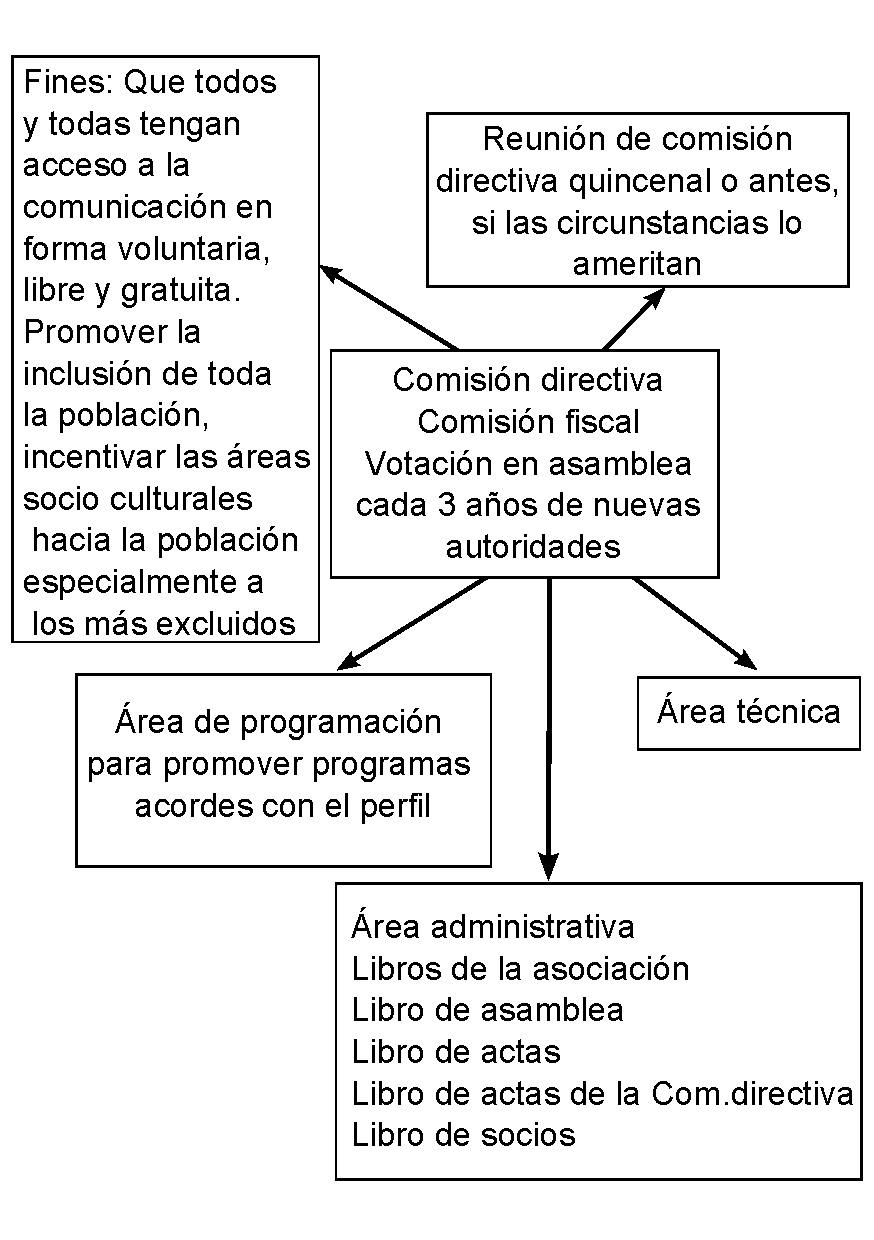
\includegraphics[scale=0.6]{./Cap/Organigramas/hela.pdf}
 % universo.pdf: 595x842 pixel, 72dpi, 20.99x29.70 cm, bb=0 0 595 842
 \caption{Organigrama de radio La Heladera, José Pedro Varela, Lavalleja.}
\end{figure}

\begin{figure}[htbp]
 \centering
 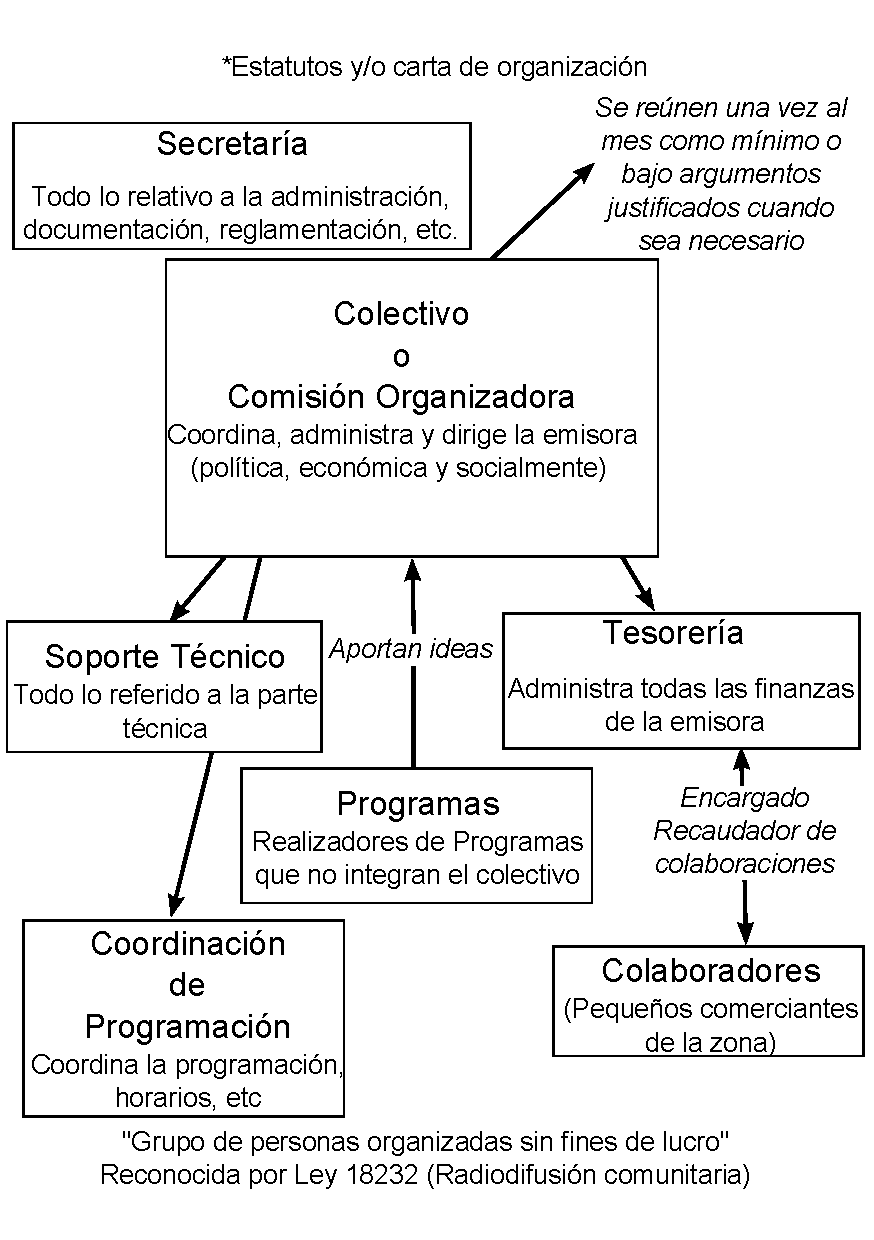
\includegraphics[scale=0.7]{./Cap/Organigramas/uni.pdf}
 % universo.pdf: 595x842 pixel, 72dpi, 20.99x29.70 cm, bb=0 0 595 842
 \caption{Organigrama de radio Universo, Montes, Canelones.}
\end{figure}

\begin{figure}[htbp]
 \centering
 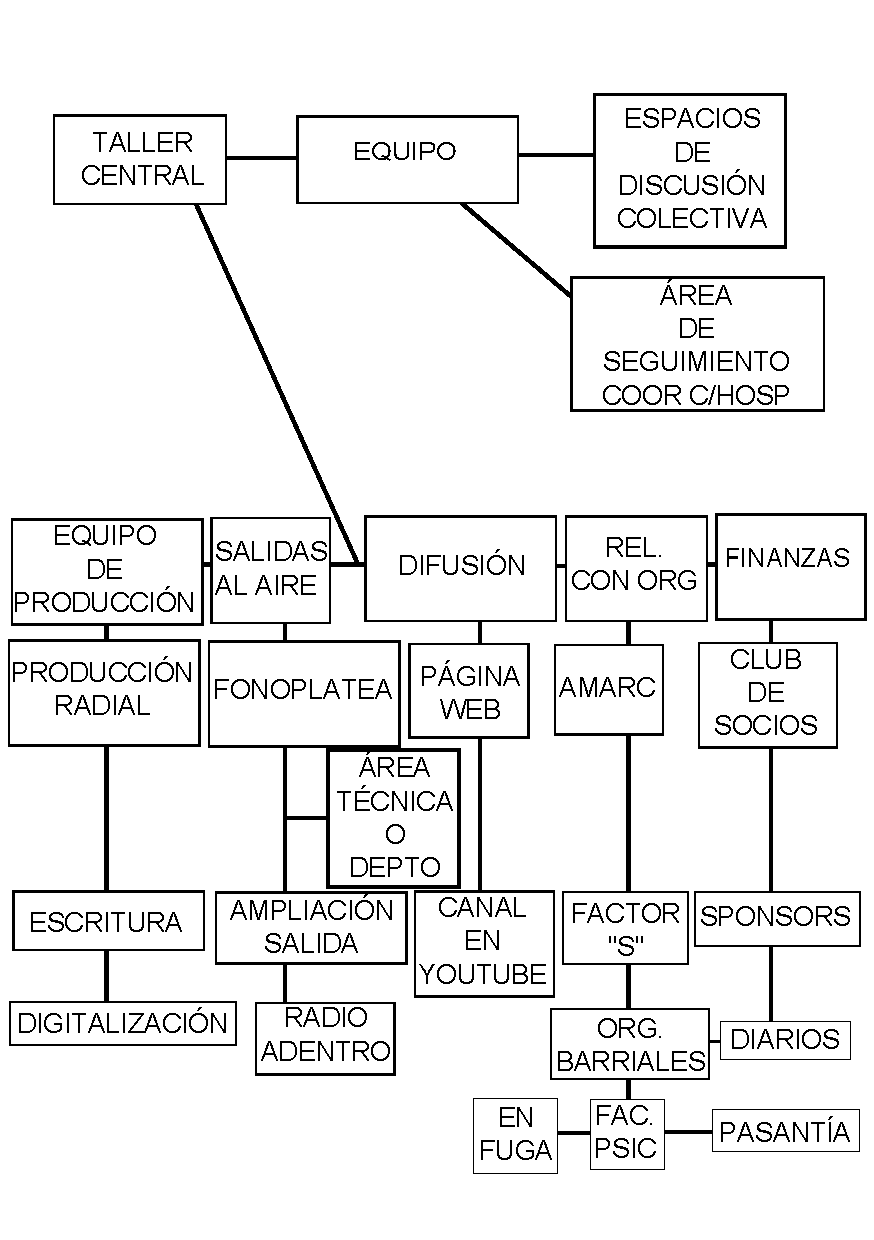
\includegraphics[scale=0.7]{./Cap/Organigramas/vilar.pdf}
 \caption{Organigrama de radio Vilardevoz, Montevideo.}
 \label{OrgVilardevoz}
\end{figure}
\newpage
\section{Elementos diferenciales}

Todas las organizaciones, tanto las asociaciones civiles como las comisiones de vecinos formadas presentan particularidades, innovaciones dentro de la estructura y por lo tanto formas de funcionamiento que se diferencian del resto y que de una u otra manera aportan al común de la red elementos diferenciales que podrían ser utilizados en beneficio de todos.\\

Algunos de estos elementos son los siguientes:\\

\textbf{Elaboración de Fines}\\

Estos fines refieren al compromiso del colectivo con la comunidad en las diferentes actividades que se realizan. Comunicación libre y gratuita, inclusión de los distintos proyectos radiales en la comunidad, actividades socioculturales, creación de espacios teatrales y musicales, etc.\\

\textbf{Inclusión de nuevos integrantes}\\

Se le provee a la persona que quiera ingresar al colectivo capacitación tanto técnica como en la propia elaboración de la propuesta radial. Asimismo se realiza un proceso de acompañamiento inicial, en el proceso de inclusión, que incluye un seguimiento del programa durante los primeros meses.\\

\textbf{Producción}\\

Se destacan los métodos de producción colectiva. Esto refiere a los contenidos tanto musicales como periodísticos con claros intereses referidos a la comunidad de la cual la radio es parte.\\

\textbf{Referentes}\\

La utilización de referentes por áreas permite un mejoramiento sustancial en las tareas diarias  ya sea en la parte técnica como en las tareas de producción radial, administrativas y de gestión.\\

\textbf{Figura de recaudador}\\

Algunas de las radios han optado por utilizar una persona que les facilite las cobranzas, tanto de la publicidad como de las cuotas sociales, que se utilizan para el financiamiento interno.\\

\textbf{Coordinadores de programación}\\

Permite integrar las grillas de programas. Trabaja en torno a los horarios y los tipos de programas que componen la grilla.\\
\chapter{Comunicación\label{Comunica}}

En este documento se presentan las diferentes estrategias de comunicación  mencionadas por los diferentes colectivos. Si bien inicialmente en la consigna se pretendió que se incluyera una evaluación sobre la funcionalidad, o los contenidos de esa información, este aspecto no fue profundizado en el material recogido. Sin embargo, éste fue tomado como insumo por la Asamblea de AMARC, donde se planteó la necesidad de conseguir dar esta discusión colectivamente, y repensar la funcionalidad de las diferentes estrategias usadas, el por qué de cada dispositivo, y los mensajes que se transmiten.\\

En relación a las estrategias de comunicación con la comunidad empleadas por los diferentes colectivos no se realiza en este documento una revisión profunda de las diferentes concepciones de relacionamiento con la comunidad o de participación comunitaria. Se presentan los diferentes mecanismos de difusión del proyecto político-comunicacional de la radio y de actividades que ésta realiza.\\

\section{Comunicación Interna}

Del material recogido se desprende que se prioriza la palabra, escuchar lo que el compañero tiene para decir, tanto en los talleres y asambleas, como en el día a día, en los aspectos organizativos. El “boca a boca”, para la transmisión de mensajes es de uso general en todas las radios.\\

Es también de uso frecuente el formato papel, tanto carteles en espacios del local radial así como carteleras. Se utilizan también otros dispositivos similares (pizarras, pizarrones) en espacios visibles del local radial, donde se indica información actualizada y relacionada tanto con actividades como con aspectos de convivencia.\\

Algunos ejemplos:\\

\textit{¿Hemos analizado la forma en que tejemos nuestra programación y nuestros programas? ¿Hemos aprovechado los recursos y potencialidades sonoras que existen en nuestra localidad para enriquecer nuestro trabajo?}

(Cartel en estudio de la Radio Horizonte, Paysandú)\\

\textit{Porque es necesario pensar en hacer otra historia, te convidamos a compartir con este colectivo. ANIMATE !!! seguro tenes algo importante pa' decir.}

(Cartelera de la Radio Utopía, Colonia Nicolich)\\

\textit{Si (el baño) hablara ¿qué diría de ti? La limpieza del baño habla de quien lo usa. El compañerismo también se mide en ello.}

(Cartel en baño del local de la Radio Horizonte, Paysandú)\\

Asimismo, a modo de registro, en las paredes de las radios hay afiches y cartelería diversa de actividades organizadas por la radio u otras organizaciones, así como también de grupos musicales y fotos de personalidades públicas referentes para el colectivo. En algunos casos hay diplomas encuadrados, o material de la red o de AMARC internacional.\\

Para actividades de la radio, en radio Gral. Artigas de Toledo, se utiliza un dispositivo de comunicación, que facilita la organización de talleres u otras actividades a realizarse colectivamente. Se realizan “Comunicados con notificación”, donde se especifica la actividad, lugar y horario, y una grilla. Allí cada integrante firma su notificación de saber la actividad, y especifica si puede participar, y en qué horario.\\

La radio misma se vuelve un medio de comunicación interna, ya que los integrantes del colectivo escuchan la radio en sus casas o trabajos. En los distintos programas se brinda información de cuestiones internas.\\

Asimismo los integrantes de las radios que permanecen más horas en las mismas (operadores, referentes de programas) se convierten en referentes en la comunicación interna.\\

Por otra parte, es de uso frecuente la telefonía como medio de comunicación entre los integrantes del colectivo. Se utilizan los teléfonos de la propia radio, los teléfonos fijos de los integrantes, así como sus celulares, tanto vía mensaje de texto o llamadas. En algunos colectivos se utiliza el correo electrónico como medio de comunicación interna, y en algún caso cuentan con una lista de distribución para los mismos.\\

Puesto que, en general, las radios están muy vinculadas al espacio local, la cercanía colabora en optimizar la comunicación: se va a la casa de los compañeros, se utiliza una suerte de comunicación “puerta a puerta”. En el caso de las radios cuyos locales se encuentran en la casa de alguno de sus integrantes, ésta sirve como espacio de encuentro (La Heladera, Radio Prado, Horizonte Max).\\

Las reuniones sistemáticas son una forma de garantizar ciertos niveles de circulación de la información relacionada a la radio y las decisiones referidas a la misma. En ocasiones, estas reuniones son semanales o quincenales, mientras que en otros la periodicidad es relativa, pudiendo ser como las mencionadas o a demanda (motivadas por asuntos de interés específico del colectivo, ingreso de nuevos integrantes).\\

Para mantener la información sistematizada se plantean ejemplos, citados como dispositivos de mucha utilidad:

\begin{itemize}
 \item \textbf{Libro de actas}. Utilizado en La Heladera, como herramienta de registro interna y con validez formal. Se deja constancia de las Asambleas, reuniones de la comisión directiva, etc.
 \item \textbf{Cuaderno de actas}. En Timbó, se deja constancia de las decisiones del colectivo en un cuaderno, pero con formalidades que le dan validez legal. Por ejemplo, se firma cruzado, cuando se anexa alguna hoja.
 \item \textbf{Actas y crónicas de las actividades realizadas}. Vilardevoz registra sus actividades en estas dos modalidades, y las sube a su web.
 \item \textbf{Cuaderno de comunicaciones}. Utilizado por Espika, donde se registra el estado del local radial al llegar, en el caso de que haya algo importante para comunicar a los compañeros que vendrán.
\end{itemize}

\section{Comunicación con la Comunidad}
En la salida al aire, se establece un contacto y comunicación permanente.\\

Se utilizan también:\\

\begin{itemize}
  \item Piques del proyecto comunicacional, o simplemente con el nombre de la emisora.
  \item Spot de programas y eventos.
  \item Spot solicitados por la propia comunidad (El Capiz). Pueden ser grabados por los propios actores implicados, o puede ser grabado por algún integrante de la radio sobre el texto que se les brinda.
\end{itemize}

Se realiza intercambio en el día a día con el vecino, a través de los diferentes programas, de correos electrónicos, del boca a boca, teléfono, mensaje de texto, encuentros casuales con la audiencia.\\

Se citan también las visitas y la participación de la audiencia en persona en los programas. Cabe destacar el singular caso de Vilardevoz, que realiza una Fonoplatea, sábado a sábado, donde se invita a participar de la salida al aire desde el Hospital Vilardebó.\\

Se mencionan asimismo salidas al barrio, para conseguir sponsor, para hablar con la audiencia, mostrar la radio.\\

Se realizan frecuentemente entrevistas a diferentes actores sociales, tanto en vivo como grabadas.\\

Por otra parte, se utilizan medios de publicidad audiovisual, realizados por los propios integrantes o a través de la  contratación de algún servicio. Se utilizan: volantes, afiches, pancartas, pegotines, pintadas en muros de la ciudad,\\

Pizarrón en la puerta del local radial, cartelería en la ruta y en el pueblo (El Capiz), publicidad rodante (Universo, La Cotorra).\\

Se utilizan medios gráficos de comunicación:\\

\begin{itemize}
  \item Boletín Sinapsis (Espika).
  \item Boletín Vilardevoz, (Vilardevoz)
  \item La Cotorra emitía un Periódico “La Jaula”, que no está ya en circulación
\end{itemize}


Otra vía de comunicación con la comunidad es a través de Internet. Varias emisoras disponen de su propia página web, donde comunican sus principios, programación, actividades y donde en algunos casos trambién se puede escuchar la radio online. Se detallan a continuación las páginas correspondientes:

\begin{itemize}
  \item El Puente: \href{http://www.lateja.org.uy/elpuente/index.html}{www.lateja.org.uy/elpuente/index.html}
  \item Prado: \href{http://www.elpradofm.net}{www.elpradofm.net}
  \item General Artigas: \href{http://radioartigas.radioteca.net}{radioartigas.radioteca.net}
  \item Horizonte: \href{http://www.horizonte989.org}{www.horizonte989.org}
  \item Horizonte Max: \href{http://horizontemax913.blogspot.com}{horizontemax913.blogspot.com}
  \item La Heladera: \href{http://laheladera.awardspace.biz/index1.html}{laheladera.awardspace.biz/index1.html}
  \item Timbó: \href{http://www.fmtimbo.ensanjose.com}{www.fmtimbo.ensanjose.com}
  \item Universo: \href{http://www.universofm.es.tl}{www.universofm.es.tl}
  \item Vilardevoz: \href{http://radiovilardevoz.wordpress.com}{radiovilardevoz.wordpress.com}
\end{itemize}

Varios colectivos utilizan sistemas de comunicación instantánea a través de internet para comunicarse con la audiencia. En algunos casos se utilizan también redes sociales, en otros colectivos el uso, el objetivo y los resultados posibles del uso de estos medios es aún objeto de discusión.\\

También se realizan diferentes tipos de eventos sociales (actividades culturales, espectáculos musicales, transmisión de Carnaval), que son considerados espacios de comunicación con la comunidad. En algunos casos a través del apoyo a actividades que ésta realiza, en otros casos desde las actividades de la propia radio.\\

En el caso de La Cotorra se participa en la elaboración y difusión de las actividades del Centro Cultural Florencio Sánchez. Esta emisora es además parte de los destinos a visitar el día del Patrimonio en el marco del Cerro Cultural.\\

Algunas emisoras festejan sus cumpleaños en algún espacio público, realizando una invitación abierta a los vecinos.\\

También se realiza apoyo solidario de actividades, o se realizan campañas de solidaridad con algún vecino. Radio Prado brinda wifi de acceso libre para las XO; Utopía lleva adelante una bolsa de trabajo.\\

Por otra parte cabe destacar que algunos colectivos han realizado proyectos de desarrollo específico con la comunidad.\\
\begin{itemize}
  \item Talleres con escuelas y liceos (La Cotorra).
  \item Primer Escuela de Rock (La Cotorra).
  \item Proyecto “Galpones”: espacio socio-cultural, cogestionado con otros organizaciones sociales que está en proceso (Espika).
  \item Aire Mojado (Fondos Concursables MEC - Espika).
  \item “El Cerro habla”: documental (Fondos PNUD-La Cotorra).
  \item “Entre jóvenes” (INJU-Insomnio)
\end{itemize}
Algunos de ellos contaron con financiamiento (ver capítulo \ref{financieros}).

En relación al contacto con otras organizaciones, se destaca la particularidad de Vilardevoz de participar en congresos, o de realizar desembarcos (presentación de la radio en otros espacios, como Facultad de Psicología).\\

Asimismo cabe destacar la participación directa en el SOCAT, como representante barrial, de La Cotorra. En este caso se establece también un acuerdo de trabajo con un pasante de comunicación del Centro Comunal Zonal 17.\\

En Impactos y Utopía hay organizaciones sindicales que tienen sus propios programas en la radio.\\

Se menciona asimismo la realización de Asambleas barriales, y otras modalidades novedosas como la participación en movilizaciones, o cortes de ruta promovidas por tema de preocupación de la comunidad (Utopía), cartelera con estado de cuenta de la radio (Universo), buzón en la puerta del local radial (El Capiz). Radio Espika ha organizado Foros Sociales en la ciudad de Santa Lucía.\\

\section{Comunicación con la Red}

En lo que respecta a la comunicación con la red se plantea la existencia de dificultades para mantener una comunicación fluida.  Se destaca que el acceso a internet de todas las radios puede generar más posibilidades de mantener un contacto más fluido. Se plantea asimismo la existencia de relacionamiento con radios comunitarias no asociadas a AMARC, en particular por cercanía geográfica.\\

Se citan la comunicación telefónica como la vía principal de comunicación. También el correo electrónico es de uso frecuente. El podcast es usado para compartir producciones con otros colectivos.\\

Se menciona asimismo las asambleas como espacio privilegiado de comunicación de la red, destacando además los espacios colectivos como los diferentes talleres de formación. Los campamentos anuales son mencionados como un espacio de comunicación importante.\\

Se hace referencia a las acciones sociales conjuntas, los dúplex entre varias emisoras, y las colaboraciones técnicas.\\

Se realizan visitas a los locales radiales de emisoras asociadas, así como intercambios entre diferentes compañeros de la mesa o las áreas de trabajo.
\chapter{Fuentes de información}

En materia de información utilizada para la salida al aire, y para la preparación de los programas, se hace un uso variado tanto en el tipo de información como en la obtención de la misma.\\

Los temas a tratar surgen en general de los propios compañeros o de sugerencias de oyentes. En algunas emisoras los temas abordados al aire, se imprimen en un boletín de la radio.\\

Se especifica a continuación diversas categorías, que resumen la variedad encontrada.\\

\section{Material gráfico}

\subsection{Diarios}

De las radios sistematizadas 13 de 15 mencionan explícitamente que utilizan los medios de prensa escritos a nivel nacional como fuente de información. Disponen de medios diversos (El País, Últimas Noticias, El Espectador, La República, Brecha, La Diaria). La Diaria es mencionada por 5 de las 15, Brecha 3 de las 15, y La República por 2 de 15, mientras que los demás medios son referenciados por única vez y por diferentes radios. En algunos colectivos se reciben los periódicos por gentileza de un kiosco cercano, que otorga el material en calidad de préstamo por unas horas.\\

Asimismo, se utilizan en algunas radios medios de prensa escritos de origen internacional.\\

Son frecuentes los diarios locales como fuente de información, 5 de 15 radios mencionan utilizarlos. Se menciona boletín CCZ 17, boletín IMM, Cosmópolis, El Tejano, Jubicerro, Visión ciudadana, San José hoy, Primera hora.\\

Sin embargo, una de las radios explicita no hacer uso del medio local, por no compartir su forma de entender el periodismo gráfico, prefiriendo entonces otras fuentes acordes a su proyecto político-comunicacional.\\

\subsection{Revistas}

Algunas radios mencionan utilizar revistas varias como fuente de información, especificando las siguientes: Revista FENAPES, SEPREDI, InfoMides, Revista Embajada de Venezuela, América XXI, Caras y Caretas, 3 puntos. En otros casos, solamente se refiere al uso de revistas en general.\\

\subsection{Libros}

Se indica el uso de libros, tanto aquellos provenientes de los propios integrantes del colectivo, como de bibliotecas zonales. Se señala también el uso de enciclopedias como material de referencia.\\

Como particularidad, Horizonte de Artigas señala que acude a lanzamientos de libros, y Espika organiza presentaciones de libros.\\

\subsection{Otros}

Por otra parte se indica el uso de materiales de AMARC, la publicación ``Cara y Señal'', así como otras publicaciones de la red.\\

Se hace referencia también al uso de los almanaques del Banco de Seguros del Estado.\\

\section{Web\label{web}}

Todas las radios actualmente tienen acceso a internet (algunas lo lograron en el marco del proyecto TICs de AMARC). De todos modos, el empleo de este recurso no es utilizado de la misma forma en todos los colectivos.\\

Se utilizan programas de mensajería instantánea (chat) o redes sociales, para comunicarse entre los integrantes del colectivo y/o para comunicarse con la comunidad.\\

Algunos colectivos poseen un mayor conocimiento de páginas que son de utilidad para su proyecto político-comunicacional, otros realizan búsquedas según la necesidad y no tienen páginas de referencia o de uso frecuente.\\

Entre las mencionadas, se pueden destacar aquellas de uso frecuente para descargar música u otros materiales:\\

\begin{itemize}
 \item \href{http://www.jamendo.com}{www.jamendo.com}
 \item \href{http://www.requecheando.com}{www.requecheando.com}
 \item \href{http://www.taringa.com}{www.taringa.com}
 \item \href{http://www.4shared.com}{www.4shared.com}
 \item \href{http://www.perrerac.org}{www.perrerac.org} (descarga de música con licencia Creative Commons)
\end{itemize}

\indent Asimismo se mencionan páginas de información general o de noticias, relacionadas con temas de interés para las radios como derechos humanos, medio ambiente, violencia doméstica, drogas, pobreza, género, sexualidad, realidades barriales, información latinoamericana, entre otros:\\

\textbf{Enciclopedia virtual}:
\href{http://www.wikipedia.org}{www.wikipedia.org}\\

\textbf{Nacionales}:
\begin{itemize}
 \item \href{http://www.montevideo.com.uy}{www.montevideo.com.uy}
 \item \href{http://www.180.com.uy}{www.180.com.uy}
 \item \href{http://www.presidencia.gub.uy}{www.presidencia.gub.uy}
 \item \href{http://www.sanjosehoy.wordpress.com}{www.sanjosehoy.wordpress.com}
 \item \href{http://www.sanjosenoticias.com.uy}{www.sanjosenoticias.com.uy}
 \item \href{http://www.paysandu.org.uy}{www.paysandu.org.uy}
\end{itemize}

\textbf{De información general}:

\begin{itemize}
 \item \href{http://www.rebelion.org}{www.rebelion.org}
 \item \href{http://www.ipsnoticias.net}{www.ipsnoticias.net}
 \item \href{http://www.jakueke.com}{www.jakueke.com}
 \item \href{http://www.pressenza.org}{www.pressenza.org}
 \item \href{http://www.indymedia.org}{www.indymedia.org}
 \item \href{http://www.amnistia.org.uy}{www.amnistia.org.uy}
 \item \href{http://www.telesurtv.net}{www.telesurtv.net}
 \item \href{http://www.idealist.org}{www.idealist.org}
\end{itemize}

Se hace mención al uso de páginas gubernamentales, sitios de organizaciones y movimientos sociales latinoamericanos, pero no aparecen especificadas.\\

Se menciona en un caso el uso de web de centros científicos y de universidades, pero no se puntualiza su forma de acceso.\\

Por último, se mencionaron aquellos sitios relacionados a AMARC y a otras Radios Comunitarias y/o online:\\

\begin{itemize}
 \item \href{http://www.amarcuruguay.org}{amarcuruguay.org}/\href{http://podcast.amarcuruguay.org}{podcast.amarcuruguay.org}
 \item \href{http://www.radialistas.net}{www.radialistas.net}
 \item \href{http://www.agenciaradioweb.com}{www.agenciaradioweb.com}
 \item \href{http://www.agenciapulsar.org}{www.agenciapulsar.org}
 \item \href{http://www.comcosur.com.uy}{www.comcosur.com.uy}
 \item \href{http://www.farco.com.ar}{www.farco.com.ar}
 \item \href{http://www.radiomundoreal.fm}{www.radiomundoreal.fm}
 \item \href{http://www.elmundo.es}{www.elmundo.es}
\end{itemize}

\section{Interna}

Se indica en este ítem aquellas fuentes de información identificadas por los colectivos como información proveniente de sus propios integrantes. Esto reúne aquel material que surge de los talleres del colectivo, de las propias experiencias de vida, y de internación, en el caso especifico de Vilardevoz. Asimismo, para esta radio en particular se referencia a la información que proviene de otros actores de la  institución Hospital Vilardebó.\\

Para otros colectivos se toma también como fuente de información los estudios particulares de sus integrantes, sus propios recursos y conocimientos.\\

\section{Desde la comunidad}

Claramente el relacionamiento con la comunidad es una fuente de información para todos los colectivos. Esto va desde el “boca a boca”, el intercambio diario con los vecinos, las propias notas que los oyentes hacen llegar al local radial o vía correo electrónico.\\

Se menciona como fuente de información básica a las “prácticas de convivencia” (pueblo en sus vínculos, los pedidos de ayuda en relación a situaciones de salud, situaciones financieras, actividades de la comunidad).\\

En El Capiz se utiliza un buzón ubicado en la puerta de la radio, de donde se extrae información.\\

Por otra parte, se hace referencia tanto a la información proveniente de integrantes de la radio que no residen actualmente en la localidad (es el caso de la Heladera y particularmente en Radio Prado, donde cuentan con una compañera en Estados Unidos, que brinda información de los uruguayos inmigrantes y organizaciones sociales por la cual ella está trabajando, siendo entonces corresponsal de la radio en el exterior).\\

Se mantiene contacto con Comisiones Barriales, Comisiones Fomento, SOCAT (Servicio de Orientación, Consulta y Articulación Territorial) y diversas organizaciones sociales. También existe una comunicación fluida con las Intendencias, Juntas Locales, Centros Comunales Zonales, Alcaldías, así como con las Instituciones Educativas de la zona. De estos contactos permanentes proviene mucha de la información que sale al aire.\\

Se señala también el intercambio en algunas radios con Federación de Cooperativas, Alcohólicos Anónimos, ULOSEV (Unidad Local de Seguridad Vial), clubes de baby fútbol, sindicatos.\\

Es importante destacar que en varias emisoras las organizaciones sociales tienen su propio espacio en la radio.\\

\section{Comunicados oficiales}

Las radios reciben con asiduidad comunicados de diferente tipo para ser transmitidos a la audiencia. Éstos provienen tanto de organizaciones sociales, instituciones locales, hasta comunicados oficiales de organismos estatales. Los mencionados son la Junta Local, Ministerio de Educación y Cultura, Administración de Servicios de Salud del Estado, Administración Nacional de Telecomunicaciones (ANTEL) y URSEC.\\

Algunas radios han logrado mayor presencia pública en la comunidad, lo que repercute al momento de ser tomadas como medio de comunicación a ser tenido en cuenta.\\

Los comunicados se reciben por vía electrónica o por correspondencia.\\

\section{Otros medios de comunicación}

Se realiza intercambio con otros medios, tanto comunitarios como comerciales y se utiliza como fuente de información tanto la televisión como la radio. En algunos casos, existe un muy buen relacionamiento con las radios comerciales, señalado principalmente en las radios del interior.\\

Particularmente se mencionó a Radio Naciones Unidas\footnote{\href{http://www.unmultimedia.org/radio/spanish}{www.unmultimedia.org/radio/spanish}}, Radio Netherlands\footnote{\href{http://www.rnw.nl/espanol}{www.rnw.nl/espanol}} y Radio France Internacional\footnote{\href{http://www.espanol.rfi.fr}{www.espanol.rfi.fr}}, como medios de comunicación extranjeros.

\section{Entrevistas}

Se realizan notas a vecinos y entrevistas diversas. En algunos casos en vivo, y en otros casos son grabadas y luego salen al aire.

\section{Música}

La música emitida es en general variada. En algunos casos buscando la diversidad, en otros intentando diferenciarse de los medios comerciales, no reproducen música comercial o cumbia, priorizando la música nacional. Se indican géneros tales como: jazz, country, clásica y tango.\\

Uno de los colectivos especifica que se accede a música a través de la compra de discos en la feria vecinal y la colaboración de los oyentes que brindan material musical. En todas las emisoras se hace referencia al material que cada radialista trae para la radio. Asimismo se realizan descargas de internet, tal como se mencionó en el apartado \ref{web}.

\section{Telecomunicaciones}

Es una fuente de información presente en todos los casos, los mensajes de textos que envía la audiencia, así como las llamadas telefónicas.\\

Se implementa generalmente la salida al aire de las llamadas telefónicas.\\

Un colectivo utiliza de forma semanal skype con una corresponsal uruguaya en el extranjero.\\
\chapter{Fundaciones de las radios}
\indent Con cada colectivo se trabajó el tema ``Historia de la red'', buscando una descripción de la trayectoria de cada uno, mediante la elaboración colectiva de una narración. En este capítulo transcribiremos textualmente lo que cada colectivo generó, aunque (por motivos de espacio) sólo se extrae lo referente a la creación de la radio, a su concepción inicial, su fundación.\\

\section*{El Capiz (Valizas)}
``Yo diría que la movida de la radio empezó con un transmisor muy elemental hecho por Daniel (hermano del Cholo) que transmitía solo enchufándole un Walkman y salíamos con una radio a ver cuántas cuadras se escuchaba.

Un vecino que frecuentaba el pueblo y formaba parte de El Capiz y tenía contactos con AMARC, nos trajo un trasmisor estéreo y creamos La Marea FM, la cual funcionó unos dos años con mucha participación, y mucha desorganización.

Algunos integrantes de aquella primera radio seguimos con la idea de hacer radio y en el año 2006, el Cholo compró otro trasmisor y empezamos con El Capiz FM 107.5.

Empezó trasmitiendo en una piecita en la casa del Cholo, sólo los viernes de noche y domingos de mañana. Con un huevito y otro equipo musical.''

\section*{Horizonte (Paysandú)}
``Nace de una inspiración de Orlando, al ver pasar por el frente de su casa un chico drogándose. Al ser parte del barrio, sintió que debía hacer algo.
Entonces nace Horizonte FM, una radio comunitaria, la primera de Paysandú, con ganas de cambiarle la cabeza a la sociedad.

Como anécdota, cuando se fundó la radio había dos nombres para ponerle: Horizonte y Ombú (haciendo referencia al árbol más antiguo del barrio). Finalmente, por votación se escogió el nombre de Horizonte.

El 29 de marzo del año 2005, la radio sale al aire por primera vez, a las 19:30, con el seudónimo de Horizonte 989, emitiéndose desde un taller, con la ayuda de Gabriel.''

\section*{La Heladera (José Pedro Varela)}
``Un grupo de soñadores Varelenses de edades y ocupaciones diversas, comparten un proyecto: crear una radio como espacio de comunicación no comercial, con fines estéticos, culturales y de información objetiva a una comunidad bombardeada por los medios masivos y para ello se lanzan a la aventura de crear una radio comunitaria. El 23 de setiembre de 2005 con un equipo básico, en el living de una casa de familia, emitiendo tan solo 8 horas por día, se inician en el viaje que hoy ya es una realidad objetiva y no un sueño. Dos arduas tareas les esperaban, conseguir un espacio físico permanente y adecuado, y obtener la personería jurídica de la Asociación Civil que debería servir de sustento legal a la radio. La Asociación Civil se llamó El Candil y se obtuvo la personería jurídica en 2008, mientras que el local lo proporcionara la educadora insigne, Maestra Bimba Vega, quien por mucho tiempo sustenta gastos esenciales para el funcionamiento de la radio desde el 2006. (...)

Un hecho anecdótico interesante lo constituye la denominación de la radio: cuando nos instalamos en el local de Bimba, una vieja casona que había sido comité político, sus puertas no cerraban bien, y ante el temor de perder los equipos, éstos se guardaban en una vieja heladera en desuso, que se cerraba con cadena y candado. Con el paso del tiempo se producían diálogos tales como: “vamos a abrir la heladera” para referirse a que iba a sacar los equipos y comenzar la emisión… de ahí el nombre de la radio La Heladera.''

\section*{Parque (La Paloma)}
``La radio comenzó a salir desde un barrio de la Paloma (barrio Parque) como fruto del interés de un grupo de personas.

Su origen es anterior a la existencia de la ley. Luego fue inscripta en el censo y hoy está autorizada a emitir pero aun no está la resolución final de la URSEC.
El grupo inicial no mantuvo el trabajo de la radio y por tanto dejo de salir al aire durante un buen tiempo (tal vez un año).

A mediados del año 2009 surgió la idea de trasladar la radio a un gimnasio y de enganchar al liceo y otros centros para trabajar en la misma. A partir de allí se involucró un grupo nuevo de gente que es la que está hoy tratando de concretar el proyecto de radio comunitaria.''

\section*{Prado (Paso de la Arena)}
``El día 31/12/04 se inicia la radio con la primer salida 10 y 10 de la noche.

El 26 de febrero de ese año el agradecimiento a la gente, en el club Caffa, superando la venta de entradas de carnaval de ese establecimiento.

En agosto se festeja el día del niño llevando a los vecinos al parque Lecocq y compartiendo una fiesta para los niños, llenando la calle en ese día.

El primer año se realiza en la calle haciendo el primer reparto de juguetes, se sigue la relación con la gente, interactuando con los vecinos en los diferentes ámbitos. Tanto en ayuda con los merenderos, así con la ayuda en sillas de ruedas y bastones hasta mesas o canastas comestibles.''

\section*{Universo (Montes)}
``Dos jóvenes DJ de Montes un día a la venida de un baile, se les ocurrió de poner una radio para pasar música. Con la ayuda del abuelo de uno de ellos armaron un trasmisor artesanal, con una antena casera.

Se hacen las pruebas técnicas y los jóvenes quedan haciendo un programa musical que tuvo mucho éxito, por ser una novedad que estaban al aire y la gente llamaba para pedir temas.

Todo fue en una pieza de la estación de AFE por colaboración del padre de uno de los jóvenes. Luego se trata de formar más programas en la radio, invitando a personas vinculadas a temas sociales de la zona.''

\section*{Insomnio (Las Piedras)}
``La radio surge en octubre de 2006, ante la necesidad de profundizar el contacto con la comunidad, relación que se venía dando desde la fundación de la ONG en el año 1993.

2006 - inicio de actividades en el domicilio de un compañero, con pocos programas, muy poco conocimiento técnico y potencialidades de un medio de comunicación masivo.

2007 - un grupo de 9 compañer@s comienzan a capacitarse para el manejo global de la radio. Se inician contactos con AMARC afiliándose a la misma.''

\section*{La Cotorra (Cerro)}
``Había una vez un grupo de 39 compañeros/as que se fueron de un proyecto de radio y fundaron «La Cotorra». Después algunos/as se fueron y otros continúan hasta hoy. La idea continúa y sigue firme, tratando de mejorar día a día.

Todos los aportes de los compañeros/as continúan. Se ha logrado una continuidad aunque las personas cambien. El proyecto va más allá de las personas que los compongan: «La Cotorra cambió de frecuencia pero no de esencia». Teniendo siempre la comunicación con la comunidad. Hemos podido crecer técnicamente y en la gestión de la radio. Gracias al esfuerzo de todos/as, el apoyo del barrio que nos reconoce como un referente. Siempre dispuestos a apoyar emprendimientos barriales, tender redes y brindar ayuda.''

\section*{Espika (Santa Lucía)}

``En un pueblito no muy lejano (a 60 kilómetros de la capital) un grupo de amigos, preocupados por las guerras, decide cambiar el mundo. Surge entonces en 2003 la idea de un colectivo “Levantad Juventud”, apoyándose en los pricipios de participación popular, apuntando a la promoción de derechos humanos, haciendo foco en la equidad de género. Utilizando como ejes centrales un boletín y una radio “pirata” como fuente de difusión. 

En 2004 trasmitiendo al mundo y sus alrededores desde un garage. En esta faceta se ingresa a AMARC. En 2005 se plantea una nueva forma de trabajo: las comisiones. Posteriormente (2006) se pasa de un garage como estudio a un almacén, generando un lugar propio del colectivo.''

\section*{General Artigas (Toledo)}
``La historia de la radio se remonta a varios años antes de que ésta hiciera su primera salida al aire, ya que desde el año 1999 un pequeño grupo de inquietos de Toledo tenía la idea de poder contar en nuestra localidad una radio comunitaria. El por qué era que en la zona no había ningún medio de comunicación local, las radios y los canales de televisión son de Montevideo o son de otras ciudades, de la capital Canelones, de Pando o de Las Piedras y acá no había nada, ni un diario ni un semanario ni una revistita ni ningún medio de ningún tipo que informara de las cosas que pasaban en la ciudad. (...) Regularmente podíamos recibir en nuestra ciudad de Toledo las emisiones de dos radios comunitarias históricas del departamento como son la FM Tapié de San Ramón y la FM del Libertador de Barros Blancos. A partir de las escuchas fuimos pensando como poder concretar un medio de comunicación, que así como esas radios referidas difundían lo propio de su localidad nosotros también pudieramos cumplir con ese objetivo en Toledo.

Es así que, a finales del año 2001, comenzamos contactos con gente que estaba en el tema, como propiamente los compañeros de esas radios comunitarias nombradas (...)
% 
% Gracias al aporte de José (), luego de hacer una evaluación local por nuestra parte de cuales eran los canales disponibles, (en aquel tiempo habían muchos canales disponibles contrariamente a los que pasa hoy en día), comenzamos con la gestión de la construcción del transmisor el cual estuvo pronto a mediados del mes de agosto. Fueron en ese momento que comenzamos a colgar nuestra señal de aire con spots como por ejemplo éste. El hecho del inminente nacimiento de un medio local causo conmoción en nuestra comunidad de Toledo y eso se esparció como un reguero de pólvora afortunadamente.

En efecto en una fecha muy importante para nuestra patria, el 25 de agosto inauguramos la radio oficialmente a las 7 de la mañana y ya contábamos con algunos programas de producción local. Es de destacar que en esos primeros tiempos la radio no contaba ni con una estructura técnica ni con una infraestructura técnica ni con una infraestructura edilicia para desarrollar programas en vivo, debido a esto y a la voluntad de un montón de gente, se crearon en Toledo alrededor de 3 (entre comillas) estudios de grabaciones montados precariamente en casas de familia donde se generaban los programas, estos se grababan en disco compacto y se emitían a través de la radio.''

\section*{Timbó (San José)}

``Timbó nace de la necesidad de expresar y compartir por medio de la palabra, historias y vivencias no conocidas en la comunidad. No es solamente el deseo de ``hacer radio'' sino el deseo de hacer algo diferente desde una radio.

¿Por qué una radio?

Porque una radio produce el rescate de la palabra menoscabada, en épocas como esta. Abre las puertas de la imaginación, estimulando la creación por parte de los escuchas de nuevas imágenes y sentidos. Promueve entonces la riqueza del intercambio y la inclusión de lo singular. Habrá tantos programas como escuchas. Es crear símbolos, sonidos, es construir y producir. Estimula el deseo de hacer y pensar, ineludibles para vivir siendo protagonistas. La carta de las radios comunitarias y ciudadanas de AMARC dice: ``la palabra nos aproxima, nos revela, nos desarrolla, nos hace mejores hombres y mujeres. La palabra, libremente expresada, nos humaniza.''

\section*{Vilardevoz (Reducto)}
``Vos sabés qué es Vilardevoz.

Es nada más ni nada menos que la voz de los sin voz. Es el gritar estar vivo y tener derecho a pesar de que la circunstancia, te exilian, a veces; de la vida, de tu familia… de vos mismo y sobre todo el camino de regreso de un barco que va de lo imposible, a lo posible. De la ``utopía'' entre comillas absurda de un mundo enajenado, discriminado y aparte de muchos al derecho humano de la ``inclusión'' social con todos los derechos que todo ser humano debe usufructuar constitucionalmente: SALUD, VIVIENDA, TRABAJO. Que son la antítesis de ENFERMEDAD, INDIGENCIA y ABANDONO.

Esos derechos, son la voz de esta radio donde al encontrar soluciones se acallan las voces y se bajan los dedos discriminadores.``

\section*{Utopía (Colonia Nicolich)}

''A mediados del año 2006 en nuestro barrio Empalme Nicolich crecía una radio comunitaria. Entre mates y empanadas salió el nombre de Utopía (utopía era un sueño inalcanzable).

De a poquito entre amigos y vecinos fuimos conociéndonos, los mismos nos fueron prestando material discográfico para difundir en nuestra modesta radio.
Se aproximaba febrero y nuestro barrio no tenía su propio desfile de carnaval, con la ayuda brindada del municipio, de las agrupaciones barriales ``101 tambores'' y ``Copacabana'' y los compañeros que se disfrazaron.``

\part{Estudio de audiencia}
\chapter{Estudio de audiencia}

\indent Uno de los objetivos del proyecto de Extensión ``Las Radios no son Ruido'' era realizar un estudio de audiencia de las radios asociadas a AMARC. Para ello, se diseñó una encuesta, tomando como base una realizada para El Puente en 2004, y realizando algunas modificaciones acordadas por los integrantes del proyecto e integrantes de la mesa de AMARC.\\

\indent Por diversas razones, sólo se realizaron encuestas en 14 radios de las 15 con las que se trabajó (en ocasiones con colaboración del colectivo de las mismas), se logró llegar a 697 encuestas. El error resultante es de +/- $5,5\%$ sobre el total de la muestra, con un nivel de fiabilidad del $95\%$. Las encuestas fueron realizadas en los meses que van desde marzo hasta agosto de 2010.\\

\indent Las radios incluidas en estudio de audiencia:
\begin{itemize}
  \item Horizonte Max (Artigas)
  \item Impactos (Salto)
  \item Horizonte (Paysandú)
  \item Parque (La Paloma)
  \item La Heladera (José Pedro Varela)
  \item Universo (Montes)
  \item Prado (Paso de la Arena)
  \item Vilardevoz (Reducto)
  \item General Artigas (Toledo)
  \item Timbó (San José)
  \item Espika (Santa Lucía)
  \item Utopía (Colonia Nicolich)
  \item La Cotorra (Cerro)
  \item Insomnio (Las Piedras)
\end{itemize}

\indent Existen algunas consideraciones metodológicas acerca del estudio de audiencia. En primer lugar, sólo se realizaron encuestas en las zonas de alcance de las radios, en el entendido de que no tiene sentido preguntar a alguien si escucha una radio que no puede sintonizar por motivos puramente geográficos. En segundo lugar, dado que el equipo del proyecto tiene sólo cuatro integrantes y que, por motivos laborales, el trabajo de campo se ejecutó en fines de semana, se contó con la colaboración de algunos integrantes de algunas radios en la realización de las encuestas. La participación de los mismos es una muestra clara de su apropiación del proyecto (no era un proyecto sólo del equipo universitario), conscientemente buscando encuestar sin tener intencionalidad en la formulación de las preguntas. De todos modos, a pesar del esfuerzo por realizar un trabajo objetivo por parte de los integrantes de las radios, no se puede descartar cierta cuota de imparcialidad, que pudo haber afectado algunos resultados.\\

\indent La encuesta está dividida en cuatro secciones:

\begin{enumerate}
     \item Informaci\'on general
     \item Radioescuchas
     \item Radios comunitarias en general
     \item Radio local
\end{enumerate}

\section{Información general}

\indent En este item, se busca categorizar la poblaci\'on auditada, a trav\'es de par\'ametros generales, como son la edad, sexo, ocupaci\'on y nivel de escolarizaci\'on. Adem\'as, es de inter\'es conocer su acceso a medios masivos de comunicaci\'on, a trav\'es de medios electr\'onicos (internet). Otra informaci\'on de utilidad es conocer si poseen radios anal\'ogicas o digitales.\\

\indent Como se puede apreciar en la tabla \ref{SexoTabla}, un 52$\%$ de las encuestas fueron realizadas a mujeres, mientras que el restante 48$\%$ a hombres.

\begin{table}[ht]
	\centering
\rowcolors{1}{gray!0}{gray!20}
		\begin{tabular}{|l|l|l|}\hline
      	\textbf{Sexo}&\textbf{Frecuencia}&\textbf{Porcentaje}\\\hline\hline
			Femenino	&	362&	52$\%$\\\hline
			Masculino 	&	335&	48$\%$\\\hline
		\end{tabular}
	  \caption{Sexo}
	  \label{SexoTabla}
\end{table}


\indent Se eligió como criterio que el mínimo de edad para encuestar era de 14 años, coincidente con lo que se realiza normalmente en los estudios de audiencia (se encuestaron personas entre 14 y 88 años).\\


\indent En el cuadro \ref{OcupaTabla}, se puede observar la ocupación de los encuestados. Existe una amplia mayoría de empleados (46$\%$), seguidos por proporciones casi iguales de estudiantes, amas de casa, jubilados y pensionistas y con negocio propio.\\

\begin{table}[htpb]
	\centering
\rowcolors{1}{gray!0}{gray!20}
		\begin{tabular}{|l|l|l|}\hline
      	\textbf{Ocupación}&\textbf{Frecuencia}&\textbf{Porcentaje}\\\hline\hline
			Empleado	&	310&	44$\%$\\\hline
			Estudiante 	&	83&	12$\%$\\\hline
			Ama de casa 	&	78&	11$\%$\\\hline
			Jubilado/Pensionista 	&	87&	12$\%$\\\hline
			Desocupado 	&	25&	4$\%$\\\hline
			Changas 	&	32&	5$\%$\\\hline
			Negocio propio 	&	61&	9$\%$\\\hline
			Independiente	&	21&	3$\%$\\\hline
		\end{tabular}
	  \caption{Ocupación}
	  \label{OcupaTabla}
\end{table}


\indent En cuanto al nivel educativo, se preguntaba por el último nivel educativo finalizado. Más de una tercera parte tiene sólo terminada la escuela, mientras que un cuarto llegó a finalizar ciclo básico y otro cuarto segundo ciclo.\\

\begin{table}[ht]
	\centering
\rowcolors{1}{gray!0}{gray!20}
		\begin{tabular}{|l|l|l|}\hline
      	\textbf{Nivel educativo}&\textbf{Frecuencia}&\textbf{Porcentaje}\\\hline\hline
			Primaria	&	233&	33$\%$\\\hline
			Ciclo Básico 	&	162&	23$\%$\\\hline
			Segundo Ciclo 	&	171&	25$\%$\\\hline
			Terciaria 	&	41&	6$\%$\\\hline
			UTU 	&	57&	8$\%$\\\hline
			Magisterio 	&	11&	2$\%$\\\hline
			Profesorado 	&	10&	2$\%$\\\hline
			Otros 	&	3&	0$\%$\\\hline			
			Sin primaria completa	&	9&	1$\%$\\\hline
		\end{tabular}
	  \caption{Último nivel educativo completo}
	  \label{EscolarTabla}
\end{table}


\indent Se le preguntó a los encuestados si tenían radio analógica (``sintonizable con perilla``) o digital (``con botones``). Un 51$\%$ tiene radio analógica y un $60\%$ digital, lo que implica que muchos tienen ambos tipos de radios. Aunque no fue cuantificado, muchos de los que tenían radio digital, en realidad era como parte de equipos de más complejidad (celulares, equipos de audio, reproductores de mp3), que entre otros dispositivos, incluyen una radio.\\

\begin{table}[htpb]
	\centering
\rowcolors{1}{gray!0}{gray!20}
		\begin{tabular}{|l|l|l|}\hline
	\textbf{Radio}&\textbf{Frecuencia}&\textbf{Porcentaje}\\\hline\hline
			Analógica	&	348&	51$\%$\\\hline
			Digital 	&	412&	60$\%$\\\hline
			No tiene radio 	&	7&	1$\%$\\\hline
		\end{tabular}
	  \caption{¿Tiene radio?}
	  \label{TieneRadioTabla}
\end{table}

\indent Se preguntó a los encuestados por el acceso a internet, es decir, si en algún momento del día tenían acceso a un equipo con conexión, independientemente si era en el hogar o en el trabajo. Casi la mitad de los mismos tiene acceso a internet, lo cual señala una gran oportunidad para las radios que emiten online, así como un mayor uso de herramientas como el correo electrónico o el chat.\\

\begin{table}[htpb]
	\centering
\rowcolors{1}{gray!0}{gray!20}
		\begin{tabular}{|l|l|l|}\hline
	\textbf{Acceso a internet}&\textbf{Frecuencia}&\textbf{Porcentaje}\\\hline\hline
			Sí	&	341&	49$\%$\\\hline
			No 	&	356&	51$\%$\\\hline
		\end{tabular}
	  \caption{¿Tiene acceso a internet?}
	  \label{AccesoInternetTabla}
\end{table}


% 	\newpage
\section{Radioescuchas}
\indent Este punto refiere a los h\'abitos de los radioescuchas. Por ejemplo, d\'ias y horarios de sintonizaci\'on, preferencias de programaci\'on y g\'eneros musicales.\\

\indent Como puede verse en el cuadro \ref{EscuchaRadioTabla1}, un 89$\%$ escucha radio comúnmente, de los cuales, la mayoría (77$\%$) escucha FM y alrededor de un tercio AM (cuadro \ref{EscuchaRadioTabla2}).\\

\begin{table}[ht]
	\centering
\rowcolors{1}{gray!0}{gray!20}
		\begin{tabular}{|l|l|l|}\hline
	\textbf{Escucha radio}&\textbf{Frecuencia}&\textbf{Porcentaje}\\\hline\hline
			Sí	&	621&	89$\%$\\\hline
			No	&	73&	10$\%$\\\hline
		\end{tabular}
	  \caption{¿Escucha radio habitualmente?}
	  \label{EscuchaRadioTabla1}
\end{table}

\begin{table}[ht]
	\centering
\rowcolors{1}{gray!0}{gray!20}
		\begin{tabular}{|l|l|l|}\hline
	\textbf{Escucha radio}&\textbf{Frecuencia}&\textbf{Porcentaje}\\\hline\hline
			AM	&	229&	33$\%$\\\hline
			FM	&	537&	77$\%$\\\hline
		\end{tabular}
	  \caption{¿Escucha radio habitualmente? ¿AM y/o FM?}
	  \label{EscuchaRadioTabla2}
\end{table}

\indent Los radioescuchas muestran tener muy integrado el hábito de escuchar radio, dado que un 70$\%$ lo hace todos los días (cuadro \ref{DiasRadioTabla}).

\begin{table}[htpb]
	\centering
\rowcolors{1}{gray!0}{gray!20}
		\begin{tabular}{|l|l|l|}\hline
	\textbf{Días que escucha radio}&\textbf{Frecuencia}&\textbf{Porcentaje}\\\hline\hline
			Entre semana	&	103&	16$\%$\\\hline
			Fin de semana	&	66&	10$\%$\\\hline
			Todos los días	&	443&	70$\%$\\\hline
			NS/NC	&	28&	4$\%$\\\hline
		\end{tabular}
	  \caption{¿Qué días escucha radio?}
	  \label{DiasRadioTabla}
\end{table}


\indent En cuanto a la distribución horaria (cuadro \ref{HorasRadioTabla}), se observa una proporción alta de gente que sólo escucha en la mañana, que es casi igual a la que escucha a toda hora. Un cuarto escucha en la tarde, un 13$\%$ en la noche y un pequeño porcentaje en la madrugada. Los porcentajes no suman 100$\%$, debido a que se podían marcar varias configuraciones distintas (mañana y tarde, mañana y noche, etc).

\begin{table}[ht]
	\centering
\rowcolors{1}{gray!0}{gray!20}
		\begin{tabular}{|l|l|l|}\hline
	\textbf{Horario}&\textbf{Frecuencia}&\textbf{Porcentaje}\\\hline\hline
			Mañana	&	224&	35$\%$\\\hline
			Tarde	&	170&	27$\%$\\\hline
			Toda hora	&	231&	36$\%$\\\hline
			Noche	&	89&	14$\%$\\\hline
			Madrugada	&	14&	2$\%$\\\hline
			NS/NC	&	24&	4$\%$\\\hline
		\end{tabular}
	  \caption{¿En qué horario escucha radio?}
	  \label{HorasRadioTabla}
\end{table}

\indent Como se aprecia en el cuadro \ref{PourquoiTabla}, los dos motivos principales de escucha son información y entretenimiento.\\

\begin{table}[ht]
	\centering
\rowcolors{1}{gray!0}{gray!20}
		\begin{tabular}{|l|l|l|}\hline
	\textbf{Motivo}&\textbf{Frecuencia}&\textbf{Porcentaje}\\\hline\hline
			Información&	316&	50$\%$\\\hline
			Entretenimiento	&	428&	67$\%$\\\hline
			Religión	&	9&	1$\%$\\\hline
			Porque le gusta	&	128&	20$\%$\\\hline
			Otros	&	15&	2$\%$\\\hline
		\end{tabular}
	  \caption{¿Para qué escucha radio?}
	  \label{PourquoiTabla}
\end{table}


% \newpage
\begin{table}[ht]
	\centering
\rowcolors{1}{gray!0}{gray!20}
		\begin{tabular}{|l|l|l|}\hline
	\textbf{}&\textbf{Frecuencia}&\textbf{Porcentaje}\\\hline\hline
			Sí	&	565&	81$\%$\\\hline
			No	&	72&	10$\%$\\\hline
			NS/NC	&	60&	9$\%$\\\hline
		\end{tabular}
	  \caption{¿Escucha programas musicales?}
	  \label{MusiqueTabla}
\end{table}

\begin{table}[ht]
	\centering
\rowcolors{1}{gray!0}{gray!20}
		\begin{tabular}{|l|l|l|}\hline
	\textbf{Géneros}&\textbf{Frecuencia}&\textbf{Porcentaje}\\\hline\hline
			Cumbia	&	194&	34$\%$\\\hline
			Rock	&	91&	16$\%$\\\hline
			Melódica	&	58&	10$\%$\\\hline
			Reggae&	32&	6$\%$\\\hline
			Metal	&	6&	1$\%$\\\hline
			Tango	&	52&	9$\%$\\\hline
			Hip hop	&	13&	2$\%$\\\hline
			Salsa	&	41&	7$\%$\\\hline
			Pop	&	26&	5$\%$\\\hline
			Jazz	&	11&	2$\%$\\\hline
			Bossa Nova	&	10&	2$\%$\\\hline
			Electrónica &	11&	2$\%$\\\hline
			Folklore &	151&	27$\%$\\\hline
			Oldies &	40&	7$\%$\\\hline
			Otros &	27&	5$\%$\\\hline
			De todo	&	157&	28$\%$\\\hline
		\end{tabular}
	  \caption{¿Qué género prefiere?}
	  \label{LesGenresTabla}
\end{table}

\newpage

\section{Radios comunitarias en general}
\indent En esta sección se pretendía determinar la opini\'on y conocimiento de los encuestados acerca de las radios comunitarias en general. Interesa conocer la imagen que tiene la poblaci\'on de las mismas, en particular, el rol social y cultural que desempe\~nan y su apertura a la participaci\'on de la comunidad.\\

\indent En relación al conocimiento de alguna radio comunitaria (cuadro \ref{ConoceTabla}), un alto porcentaje de los encuestados señala conocer alguna radio comunitaria.\\
\begin{table}[ht]
	\centering
\rowcolors{1}{gray!0}{gray!20}
		\begin{tabular}{|l|l|l|}\hline
	\textbf{}&\textbf{Frecuencia}&\textbf{Porcentaje}\\\hline\hline
			Sí	&	482&	69$\%$\\\hline
			No	&	215&	31$\%$\\\hline
		\end{tabular}
	  \caption{¿Conoce alguna radio comunitaria?}
	  \label{ConoceTabla}
\end{table}

\indent Luego de preguntar si conocía una radio comunitaria, se preguntaba acerca si escuchaba radios de la zona, y el por qué de dicha elección.
\begin{table}[ht]
	\centering
\rowcolors{1}{gray!0}{gray!20}
		\begin{tabular}{|l|l|l|l|}\hline
	\textbf{}&\textbf{¿Por qué?}&\textbf{Frecuencia}&\textbf{Porcentaje}\\\hline\hline
			Sí	&&	367&	77$\%$\\\hline
				&Por información&	115&	24$\%$\\\hline
				&Militancia&	18&	4$\%$\\\hline
				&Porque es de la zona&	101&	21$\%$\\\hline
				&Porque le gusta&	123&	26$\%$\\\hline
				&Entretenimiento&	144&	30$\%$\\\hline\hline
			No	&&	109&	23$\%$\\\hline
				&No coinciden horarios&	12&	3$\%$\\\hline
				&No logra sintonizarla&	14&	3$\%$\\\hline
				&No le gusta&	30&	6$\%$\\\hline
		\end{tabular}
	  \caption{¿Escucha la radio de su zona?}
	  \label{LaEscuchaTabla}
\end{table}

\newpage

\newpage

\indent Las siguientes preguntas correspondían a una valoración del rol de las radios comunitarias, tanto a la hora de aportar información (cuadro \ref{InfoLocalTabla}), integrar a los vecinos (cuadro \ref{IntegraVecinosTabla}), promocionar actividades socio-culturales (cuadro \ref{ActSocioCultTabla}) y contribuir al desarrollo de la comunidad local (cuadro \ref{DesarrolloComunidadLocalTabla}).\\
\begin{table}[ht]
	\centering
\rowcolors{1}{gray!0}{gray!20}
		\begin{tabular}{|l|l|l|}\hline
	\textbf{}&\textbf{Frecuencia}&\textbf{Porcentaje}\\\hline\hline
			Sí	&	360&	52$\%$\\\hline
			No	&	46&	7$\%$\\\hline
			NS/NC	&	291&	42$\%$\\\hline
		\end{tabular}
	  \caption{¿Cree que aportan información local?}
	  \label{InfoLocalTabla}
\end{table}


\begin{table}[ht]
	\centering
\rowcolors{1}{gray!0}{gray!20}
		\begin{tabular}{|l|l|l|}\hline
	\textbf{}&\textbf{Frecuencia}&\textbf{Porcentaje}\\\hline\hline
			Sí	&	357&	51$\%$\\\hline
			No	&	50&	7$\%$\\\hline
			NS/NC	&	290&	42$\%$\\\hline
		\end{tabular}
	  \caption{¿Cree que ayudan a integrar a los vecinos?}
	  \label{IntegraVecinosTabla}
\end{table}


\begin{table}[ht]
	\centering
\rowcolors{1}{gray!0}{gray!20}
		\begin{tabular}{|l|l|l|}\hline
	\textbf{}&\textbf{Frecuencia}&\textbf{Porcentaje}\\\hline\hline
			Sí	&	356&	51$\%$\\\hline
			No	&	41&	6$\%$\\\hline
			NS/NC	&	300&	43$\%$\\\hline
		\end{tabular}
	  \caption{¿Cree que promocionan actividades socio-culturales?}
	  \label{ActSocioCultTabla}
\end{table}

\begin{table}[ht]
	\centering
\rowcolors{1}{gray!0}{gray!20}
		\begin{tabular}{|l|l|l|}\hline
	\textbf{}&\textbf{Frecuencia}&\textbf{Porcentaje}\\\hline\hline
			Sí	&	273&	39$\%$\\\hline
			No	&	24&	3$\%$\\\hline
			NS/NC	&	400&	57$\%$\\\hline
		\end{tabular}
	  \caption{¿Cree que contribuyen con el desarrollo de la comunidad local?}
	  \label{DesarrolloComunidadLocalTabla}
\end{table}

\indent Explícitamente se preguntaba acerca de qué hacer con las radios comunitarias. Aunque sólo 3 personas se mostraron contrarios a las mismas, existe un 55$\%$ que no tiene opinión respecto al tema. Dentro de los que respondieron ''Otros``, algunos explicitaron que se debería dar más apoyo a las radios comunitarias (en particular, económico), mientras que otros plantearon que no todas cumplen con su rol comunitario o que se debería mejorar la formación del personal de las mismas (aspecto comunicativo).\\
\begin{table}[ht]
	\centering
\rowcolors{1}{gray!0}{gray!20}
		\begin{tabular}{|l|l|l|}\hline
	\textbf{}&\textbf{Frecuencia}&\textbf{Porcentaje}\\\hline\hline
			Promocionarlas	&	383&	42$\%$\\\hline
			Clausurarlas	&	3&	0$\%$\\\hline
			Otros	&	21&	3$\%$\\\hline
			NS/NC	&	290&	55$\%$\\\hline
		\end{tabular}
	  \caption{¿Qué se debería hacer con las radios comunitarias?}
	  \label{QuoiFaireTabla}
\end{table}

\indent Las siguientes preguntas buscaban saber si la gente tiene conocimiento de que puede participar en una radio comunitaria (cuadro \ref{SabePuedeParticiparTabla}) y si le interesa (cuadro \ref{LinteresaParticiparTabla}). Poco más de una tercera parte sabe que puede participar, mientras que menos de un cuarto se muestra interesado en hacerlo.\\
\begin{table}[ht]
	\centering
\rowcolors{1}{gray!0}{gray!20}
		\begin{tabular}{|l|l|l|}\hline
	\textbf{}&\textbf{Frecuencia}&\textbf{Porcentaje}\\\hline\hline
			Sí	&	242&	35$\%$\\\hline
			No	&	74&	11$\%$\\\hline
			NS/NC	&	381&	55$\%$\\\hline
		\end{tabular}
	  \caption{¿Sabe que puede participar?}
	  \label{SabePuedeParticiparTabla}
\end{table}

\begin{table}[ht]
	\centering
\rowcolors{1}{gray!0}{gray!20}
		\begin{tabular}{|l|l|l|}\hline
	\textbf{}&\textbf{Frecuencia}&\textbf{Porcentaje}\\\hline\hline
			Sí	&	159&	23$\%$\\\hline
			No	&	150&	22$\%$\\\hline
			NS/NC	&	388&	56$\%$\\\hline
		\end{tabular}
	  \caption{¿Le interesa participar?}
	  \label{LinteresaParticiparTabla}
\end{table}

Luego se preguntaba el por qué de la elección (por qué le interesaba o no participar en una radio comunitaria). Dado que la respuesta era abierta, no se pueden establecer estadísticas al respecto. Algunas respuestas que se repetían por el no, señalaban la ''falta de tiempo'', ''falta de experiencia'' o de ''capacitación'', edad (avanzada), ''timidez'' o ''vergüenza''. Por la afirmativa, se señala el ''gusto por la radio``, el ''querer comunicar a la gente``, ''aportar a la comunidad``, ''por entretenimiento``.
\newpage
\section{Análisis de datos}

\indent Cruzando datos entre varias preguntas, se buscó sacar algunos indicadores de interés, que permitan a las radios conocer mejor a su público, así como diseñar estrategias para lograr llegar a otros miembros de la comunidad. Asimismo, la tabla de datos de la encuesta se encuentra disponible para los integrantes de las radios participantes del proyecto, en formato abierto (openoffice), de modo tal que ellos mismos puedan realizar más análisis.\\

\indent En primer lugar, se pueden apreciar algunos indicadores en el cuadro \ref{VariosIndicadoresEdadTabla}. En particular, el sexo de los encuestados, el acceso a internet y el conocimiento de al menos una radio comunitaria, por franja etaria. El conocimiento de radios comunitarias (sólo conocimiento, que no implica necesariamente la escucha), es inversamente proporcional a la edad. De todos modos, se puede visualizar que las radios comunitarias son ampliamente conocidas por la población.\\

\begin{table}[htpb]
	\centering
\rowcolors{1}{gray!0}{gray!20}
		\begin{tabular}{|p{1.3cm}|p{2cm}|p{1.6cm}|p{1.6cm}|p{1.6cm}|}\hline
      \textbf{Edades}&\textbf{Encuestados}&\textbf{Sexo femenino}&\textbf{Acceso a internet}&\textbf{¿Conoce radio comunitaria?}\\
\hline\hline
			14 a 29	&	224 (32$\%$)&50$\%$&63$\%$&75$\%$\\\hline
			30 a 49 	&	263 (38$\%$)&54$\%$&53$\%$&70$\%$\\\hline
			50 a 88 	&	210 (30$\%$)&50$\%$&30$\%$&61$\%$\\\hline\hline
			\textbf{Total}	&\textbf{697 (100$\%$)}&\textbf{52$\%$}&\textbf{49$\%$}&\textbf{69$\%$}\\\hline
		\end{tabular}
	  \caption{Algunos indicadores: género, acceso a internet y conocimiento de una radio comunitaria, por franja etaria.}
	  \label{VariosIndicadoresEdadTabla}
\end{table}

\indent En el cuadro \ref{SabePuedeParticiparEdadTabla}, sólo se analizan aquellos que dicen conocer al menos una radio comunitaria, también por franja etaria. Se nota que los sujetos de la franja etaria entre 30 y 49 años es la que menos manifiesta que sabe que puede participar del colectivo de una radio comunitaria, y también son los que menos interés muestran en participar. Muchos de los encuestados manifestaron no tener tiempo disponible para hacerlo, lo que corresponde a que toda la población entre 30 y 49 se encuentra en edad de trabajar.\\

\begin{table}[htpb]
	\centering
\rowcolors{1}{gray!0}{gray!20}
		\begin{tabular}{|p{1.5cm}|p{4cm}|p{3.8cm}|}\hline
      \textbf{Edades}&\textbf{De los que conocen, ¿sabe que puede participar?}&\textbf{De los que conocen, ¿le interesa participar}\\\hline\hline
			14 a 29	&	56$\%$&33$\%$\\\hline
			30 a 49 	&	45$\%$&29$\%$\\\hline
			50 a 88 	&	48$\%$&34$\%$\\\hline\hline
			\textbf{Total}	&\textbf{50$\%$}&\textbf{33$\%$}\\\hline
		\end{tabular}
	  \caption{¿Sabe que usted puede participar en una radio comunitaria? ¿Le interesa? Por franja etaria, sólo para los que respondieron conocer al menos una radio comunitaria.}
	  \label{SabePuedeParticiparEdadTabla}
\end{table}

\indent Se analizó la relación entre el conocimiento de radios comunitarias y el nivel educativo (cuadro \ref{EducativoParticipaTabla}). Aunque, en general, se puede ver que existe una correlación positiva entre nivel educativo y conocimiento de radios, existe una anomalía en el caso de los que dicen haber terminado educación terciaria (y no profesorado ni magisterio), que muestran tener un nivel de conocimiento inferior. Las siguientes columnas dan cuenta del porcentaje de personas que, conociendo al menos una radio comunitaria, saben que pueden participar y les interesa.\\

\begin{table}[htpb]
	\centering
\rowcolors{1}{gray!0}{gray!20}
		\begin{tabular}{|p{1.5cm}|p{1.5cm}|p{2cm}|p{2cm}|p{2cm}|}\hline
      \textbf{\begin{small}Último nivel educativo completo\end{small}}&\textbf{\begin{small}Porcentaje\end{small}}&\textbf{\begin{small}¿Conoce alguna radio comunitaria?\end{small}}&\textbf{\begin{small}De los que conocen, ¿sabe que puede participar?\end{small}}&\textbf{\begin{small}De los que conocen, ¿le interesa participar?\end{small}}\\
\hline\hline
			Primaria	&	33$\%$&65$\%$&54$\%$&34$\%$\\\hline
			Ciclo básico 	&	23$\%$&71$\%$&63$\%$&36$\%$\\\hline
			Segundo ciclo 	&	25$\%$&74$\%$&43$\%$&24$\%$\\\hline
			Magisterio 	&	2$\%$&82$\%$&49$\%$&33$\%$\\\hline
			Profesorado 	&	1$\%$&80$\%$&56$\%$&25$\%$\\\hline
			UTU 	&	5$\%$&79$\%$&38$\%$&29$\%$\\\hline
			Terciaria 	&	6$\%$&61$\%$&28$\%$&48$\%$\\\hline
			Otros	&	2$\%$&17$\%$&46$\%$&50$\%$\\\hline\hline
			\textbf{Promedio}	&--	&\textbf{69$\%$}&\textbf{50$\%$}&\textbf{33$\%$}\\\hline
		\end{tabular}
	  \caption{Conocimiento de radios comunitarias e interés en participar de las mismas, según último nivel educativo finalizado.}
	  \label{EducativoParticipaTabla}
\end{table}

\indent El cuadro \ref{OcupaParticipaTabla} es similar al anterior, aunque por ocupación laboral y no por nivel educativo.\\

\begin{table}[htpb]
	\centering
\rowcolors{1}{gray!0}{gray!20}
		\begin{tabular}{|p{1.7cm}|p{1.3cm}|p{2cm}|p{2cm}|p{2cm}|}\hline
      \textbf{\begin{small}Ocupación\end{small}}&\textbf{\begin{small}Porcentaje\end{small}}&\textbf{\begin{small}¿Conoce alguna radio comunitaria?\end{small}}&\textbf{\begin{small}De los que conocen, ¿sabe que puede participar?\end{small}}&\textbf{\begin{small}De los que conocen, ¿le interesa participar?\end{small}}\\
\hline\hline
			Ama de casa	&	11$\%$&69$\%$&43$\%$&20$\%$\\\hline
			Changas 	&	5$\%$&73$\%$&37$\%$&29$\%$\\\hline
			Desocupado 	&	3$\%$&75$\%$&56$\%$&22$\%$\\\hline
			Empleado 	&	44$\%$&69$\%$&54$\%$&38$\%$\\\hline
			Estudiante 	&	12$\%$&79$\%$&62$\%$&35$\%$\\\hline
			Independiente 	&	3$\%$&62$\%$&46$\%$&46$\%$\\\hline
			Jubilado / Pensionista 	&	12$\%$&52$\%$&49$\%$&38$\%$\\\hline
			Negocio propio	&	9$\%$&75$\%$&28$\%$&17$\%$\\\hline\hline
			\textbf{Promedio}	&--	&\textbf{69$\%$}&\textbf{50$\%$}&\textbf{33$\%$}\\\hline
		\end{tabular}
	  \caption{¿Sabe que usted puede participar en una radio comunitaria? ¿Le interesa? Por ocupación. Sólo para los que respondieron conocer al menos una radio comunitaria.}
	  \label{OcupaParticipaTabla}
\end{table}


\indent El cuadro \ref{SabePuedeParticiparSexoTabla} es similar a los anteriores, pero contemplando el aspecto de género. Los hombres tienen un mayor conocimiento de radios comunitarias (9$\%$ mayor al de las mujeres), aunque entre los que conocen existe una mayor homogeneidad (siempre con predominio masculino).
\begin{table}[htpb]
	\centering
\rowcolors{1}{gray!0}{gray!20}
		\begin{tabular}{|p{1.5cm}|p{2.2cm}|p{3cm}|p{2.8cm}|}\hline
      \textbf{Sexo}&\textbf{¿Conoce alguna radio comunitaria?}&\textbf{De los que conocen, ¿sabe que puede participar?}&\textbf{De los que conocen, ¿le interesa participar}\\\hline\hline
			Femenino&	65$\%$&48$\%$&31$\%$\\\hline
			Masculino 	&	74$\%$&52$\%$&34$\%$\\\hline\hline
			\textbf{Total}	&\textbf{69$\%$}&\textbf{50$\%$}&\textbf{33$\%$}\\\hline
		\end{tabular}
	  \caption{¿Sabe que usted puede participar en una radio comunitaria? ¿Le interesa? Por sexo, sólo para los que respondieron conocer al menos una radio comunitaria.}
	  \label{SabePuedeParticiparSexoTabla}
\end{table}
\chapter{Conclusiones}

El proyecto fue concebido como un proyecto estudiantil de extensión universitaria, lo cual puede apreciarse de acuerdo a sus objetivos y a su metodología de trabajo. A lo largo de todo el proyecto se buscó la participación activa de los colectivos, tanto en la generación de insumos para la sistematización de saberes, como para la evaluación crítica. Se logró una apropiación del proyecto por parte de la mayoría de los colectivos, lo que implica que el resultado final del mismo no es un producto exclusivo del equipo universitario, sino que es una construcción conjunta.\\

Asimismo, al trabajar sobre los aspectos que hacen a la gestión de las radios, se construyó un registro del estado de situación de cada una de ellas. Se hizo patente que la sistematización tenía valor desde el punto de vista histórico, dado que resume el panorama de las radios asociadas a AMARC en una coyuntura muy particular, de transición de una etapa de ilegalidad a otra, donde las radios adquieren derechos y obligaciones desde el punto de vista jurídico.\\

Además, aunque la intención original era que el producto del objetivo específico de sistematización de saberes fuera una especie de “manual de radiodifusión, para y por radialistas”, finalmente resultó ser demasiado ambicioso. La metodología de trabajo con cada colectivo, implicaba cubrir en una sola instancia muchos de los aspectos de la gestión de las radios, desde lo técnico a lo comunicacional, desde los recursos financieros a lo organizativo. De cada colectivo se logró obtener una visión global, validada como representativa en la instancia de plenario local. Pero, la amplitud de los temas impidió ahondar mucho en cada punto, con lo cual más que manual se terminó generando un conjunto de documentos con el estado de situación de las radios. Quizá también se puede diagnosticar que se partió de una hipótesis errónea en la formulación del proyecto, la cual era que los integrantes de las radios eran conscientes de los saberes que tenían. La experiencia de años de trabajo genera aprendizajes, pero estos pueden ser tan internalizados por los actores, que pueden llegar a pasar al terreno de lo cotidiano y no relevante.\\

Sin lugar a dudas, el estudio de audiencia es un hito en la historia de las radios comunitarias de Uruguay, dado que es el primer trabajo de alcance nacional en el tema.\\

Se puede discutir hasta qué punto se logró aportar en el proceso de fortalecimiento de las radios. El estudio de audiencia, con sus salvedades metodológicas, constituye un insumo fundamental para diseñar estrategias comunicacionales por parte de la red. Cabe destacar que, además de los resultados de cada pregunta, AMARC cuenta con la digitalización de todas las encuestas (una tabla, en formato .ods), lo que le permite realizar cruzamientos entre los puntos de las mismas, generando nuevas lecturas de la información relevada. En cuanto al objetivo de sistematización y colectivización de saberes, aunque los documentos generados no tienen la profundidad inicialmente pretendida, tienen el valor de servir como mojón en el proceso de fortalecimiento. Presentan un estado de situación de las radios a nivel nacional, en un amplio rango de temas, siendo un insumo importante para la toma de decisiones de la red. Ésa fue la evaluación que realizaron los participantes del taller nacional, que además valoraron mucho que el producto de la sistematización del relevamiento fuera colectivizado, para su edición crítica y participativa.
% \bibliographystyle{ieeetr}

% \bibliography{Bibliografia/bib7}

% \appendix
% \appendix
% \chapter*{Apéndice}
\section*{Deshabilitar la reproducción automática de dispositivos USB}
\textbf{Para Windows XP:}

\begin{enumerate}
  \item Menú Inicio $\rightarrow$ Ejecutar
  \item Escribir: \textit{gpedit.msc} y pulsar \textit{Enter}
  \item En el árbol de la izquierda, seguir esta ruta:
  \item Directiva de equipo local $\rightarrow$ Configuración del equipo $\rightarrow$ Plantillas administrativas $\rightarrow$ Sistema
  \item En la ventana de la derecha, bajar hasta \textit{Desactivar reproducción automática} (doble click)
  \item Clickear en \textit{Habilitar} y elegir la opción \textit{Desactivar reproducción automática en: Todas las unidades}
\end{enumerate}


\textbf{Para Windows 7:}

\begin{enumerate}
  \item Inicio $\rightarrow$ Panel de Control: Hardware y sonido $\rightarrow$ Reproducción automática
  \item Deshabilitar todas las opciones
\end{enumerate}

\end{document}